
\documentclass{article} % For LaTeX2e
\usepackage{iclr2027_conference,times}

% Optional math commands from https://github.com/goodfeli/dlbook_notation.
\input{math_commands.tex}

\usepackage{hyperref}
\usepackage{url}

% user add
\usepackage{wrapfig}
\usepackage{graphicx}
\usepackage{booktabs}
\usepackage{multirow}

% Table typography: compact, ICLR-consistent spacing
\setlength{\tabcolsep}{4pt}        % tighter column padding (default 6pt)
\renewcommand{\arraystretch}{1.15} % slightly airy row height
\setlength{\abovecaptionskip}{8pt}
\setlength{\belowcaptionskip}{5pt} % gap between top caption and tabular

% Float placement: reduce large inter-paragraph gaps caused by deferred
% figures/tables (ICLR template ships with conservative defaults).
\renewcommand{\topfraction}{0.95}
\renewcommand{\bottomfraction}{0.85}
\renewcommand{\textfraction}{0.06}
\renewcommand{\floatpagefraction}{0.85}
\setcounter{topnumber}{3}
\setcounter{bottomnumber}{2}
\setcounter{totalnumber}{5}
\raggedbottom

\title{Not All Errors Matter: Semantic-Aware Silent Data Corruption Detection for Large Language Models}

% Authors must not appear in the submitted version. They should be hidden
% as long as the \iclrfinalcopy macro remains commented out below.
% Non-anonymous submissions will be rejected without review.

\author{
Duo Chai$^{1}$ \quad
Cheng Liu$^{3}$ \quad
Rengang Zhang$^{2}$ \quad
Shuhuai Wang$^{1}$ \\
\bfseries Songwei Pei$^{1}$\thanks{Corresponding author: peisongwei@bupt.edu.cn} \quad
Long Cheng$^{3}$ \quad
Shangguang Wang$^{1}$ \\[2pt]
$^{1}$School of Computer Science (National Pilot Software Engineering School),\\
Beijing University of Posts and Telecommunications \\
$^{2}$Institute of Computing Technology, Chinese Academy of Sciences \\
$^{3}$School of Control and Computer Engineering, North China Electric Power University \\
\texttt{\{chaiduo,wangshuhuai,sgwang\}@bupt.edu.cn} \quad
\texttt{zhangrengang23z@ict.ac.cn} \\
\texttt{\{liucheng,lcheng\}@ncepu.edu.cn}
}

% The \author macro works with any number of authors. There are two commands
% used to separate the names and addresses of multiple authors: \And and \AND.
%
% Using \And between authors leaves it to \LaTeX{} to determine where to break
% the lines. Using \AND forces a linebreak at that point. So, if \LaTeX{}
% puts 3 of 4 authors names on the first line, and the last on the second
% line, try using \AND instead of \And before the third author name.

\newcommand{\fix}{\marginpar{FIX}}
\newcommand{\new}{\marginpar{NEW}}

%\iclrfinalcopy % Uncomment for camera-ready version, but NOT for submission.
\begin{document}


\maketitle

\begin{abstract}
Large Language Models (LLMs) are increasingly deployed in safety-critical applications such as autonomous driving and remote sensing, yet their inference remains vulnerable to Silent Data Corruption (SDC) caused by GPU soft errors. 
We observe that the majority of hardware faults are naturally masked by the model, while a small fraction induces significant semantic deviations. Moreover, the magnitude of numerical anomalies in activations does not strictly correlate with the degree of semantic corruption in outputs, rendering conventional numerical-threshold approaches inadequate—they struggle to detect critical faults reliably while incurring substantial unnecessary detection overhead. 
To address this, we propose SIEVE, a lightweight, semantic-aware soft-error detection framework for LLMs. SIEVE orthogonally projects the self-attention outputs of adjacent decoder layers into a low-dimensional space, and trains a Nominal Inter-Layer Predictor on clean execution traces to model the nominal mapping between adjacent layers. At inference time, the deviation of actual outputs from the predicted mapping is aggregated into a Discrepancy Profile, which is fed to a lightweight XGBoost classifier to identify Significant SDC events. 
Across three LLMs and three VQA benchmarks, SIEVE achieves 96.38\% precision, 91.49\% recall, and 93.78\% F1 on the primary evaluation set, with a false positive rate (FPR) of only 0.11\%. Compared with existing representative SDC detection baselines, SIEVE improves F1 by 11.38 percentage points while introducing an average end-to-end overhead of only 6.65\%.
\end{abstract}

\section{Introduction}
\label{sec:intro}
In recent years, Large Language Models (LLMs), with their strong reasoning and generation capabilities, have been increasingly deployed in safety-critical domains such as autonomous driving
\cite{sima2024drivelm,tian2024drivevlm}, remote sensing analysis\cite{wang2025disasterm3}, medical diagnosis\cite{alsabbagh2025minimedgpt}, and industrial fault diagnosis \cite{chen2025faultgpt}. These models typically rely on large-scale GPUs or other AI accelerators, whose execution is susceptible to transient hardware faults induced by cosmic rays, voltage fluctuations, and device aging\cite{wang2023understanding,he2023understanding}. Such faults can silently alter computational results without triggering any system exception, forming Silent Data Corruption (SDC). Enterprises such as Meta and Google have reported the reliability challenges posed by SDC in large-scale GPU cluster operations \cite{grattafiori2024llama,vallin2025silent}. To address this, the Open Compute Project (OCP) established the Server Component Resilience Workstream, uniting Meta, Google, NVIDIA, and other companies to study SDC. Its whitepaper on SDC in AI explicitly points out that, in large-scale inference, SDC pollutes massive inference results and disrupts downstream task decisions, and that inference-side SDC further compromises data integrity and degrades model effectiveness \cite{ocp2025sdc}. SDC therefore remains a serious safety hazard in model inference scenarios.

To investigate the impact of SDC on LLM outputs, we conduct extensive fault injection experiments, with results shown in Figure~\ref{fig:1}. Figures~\ref{fig:1}a and b show cases where the SDC does not change the semantics of the output and thus does not alter the model's decision; in contrast, Figures~\ref{fig:1}c and d show faulty outputs with severe semantic deviations that substantially affect the model's decision. We define SDCs that induce such significant semantic deviations as \textbf{Significant SDCs}; in safety-critical scenarios such as autonomous driving, this class of errors may cause severe consequences and is therefore the detection target of this work.

\begin{figure}[!ht]
\centering
    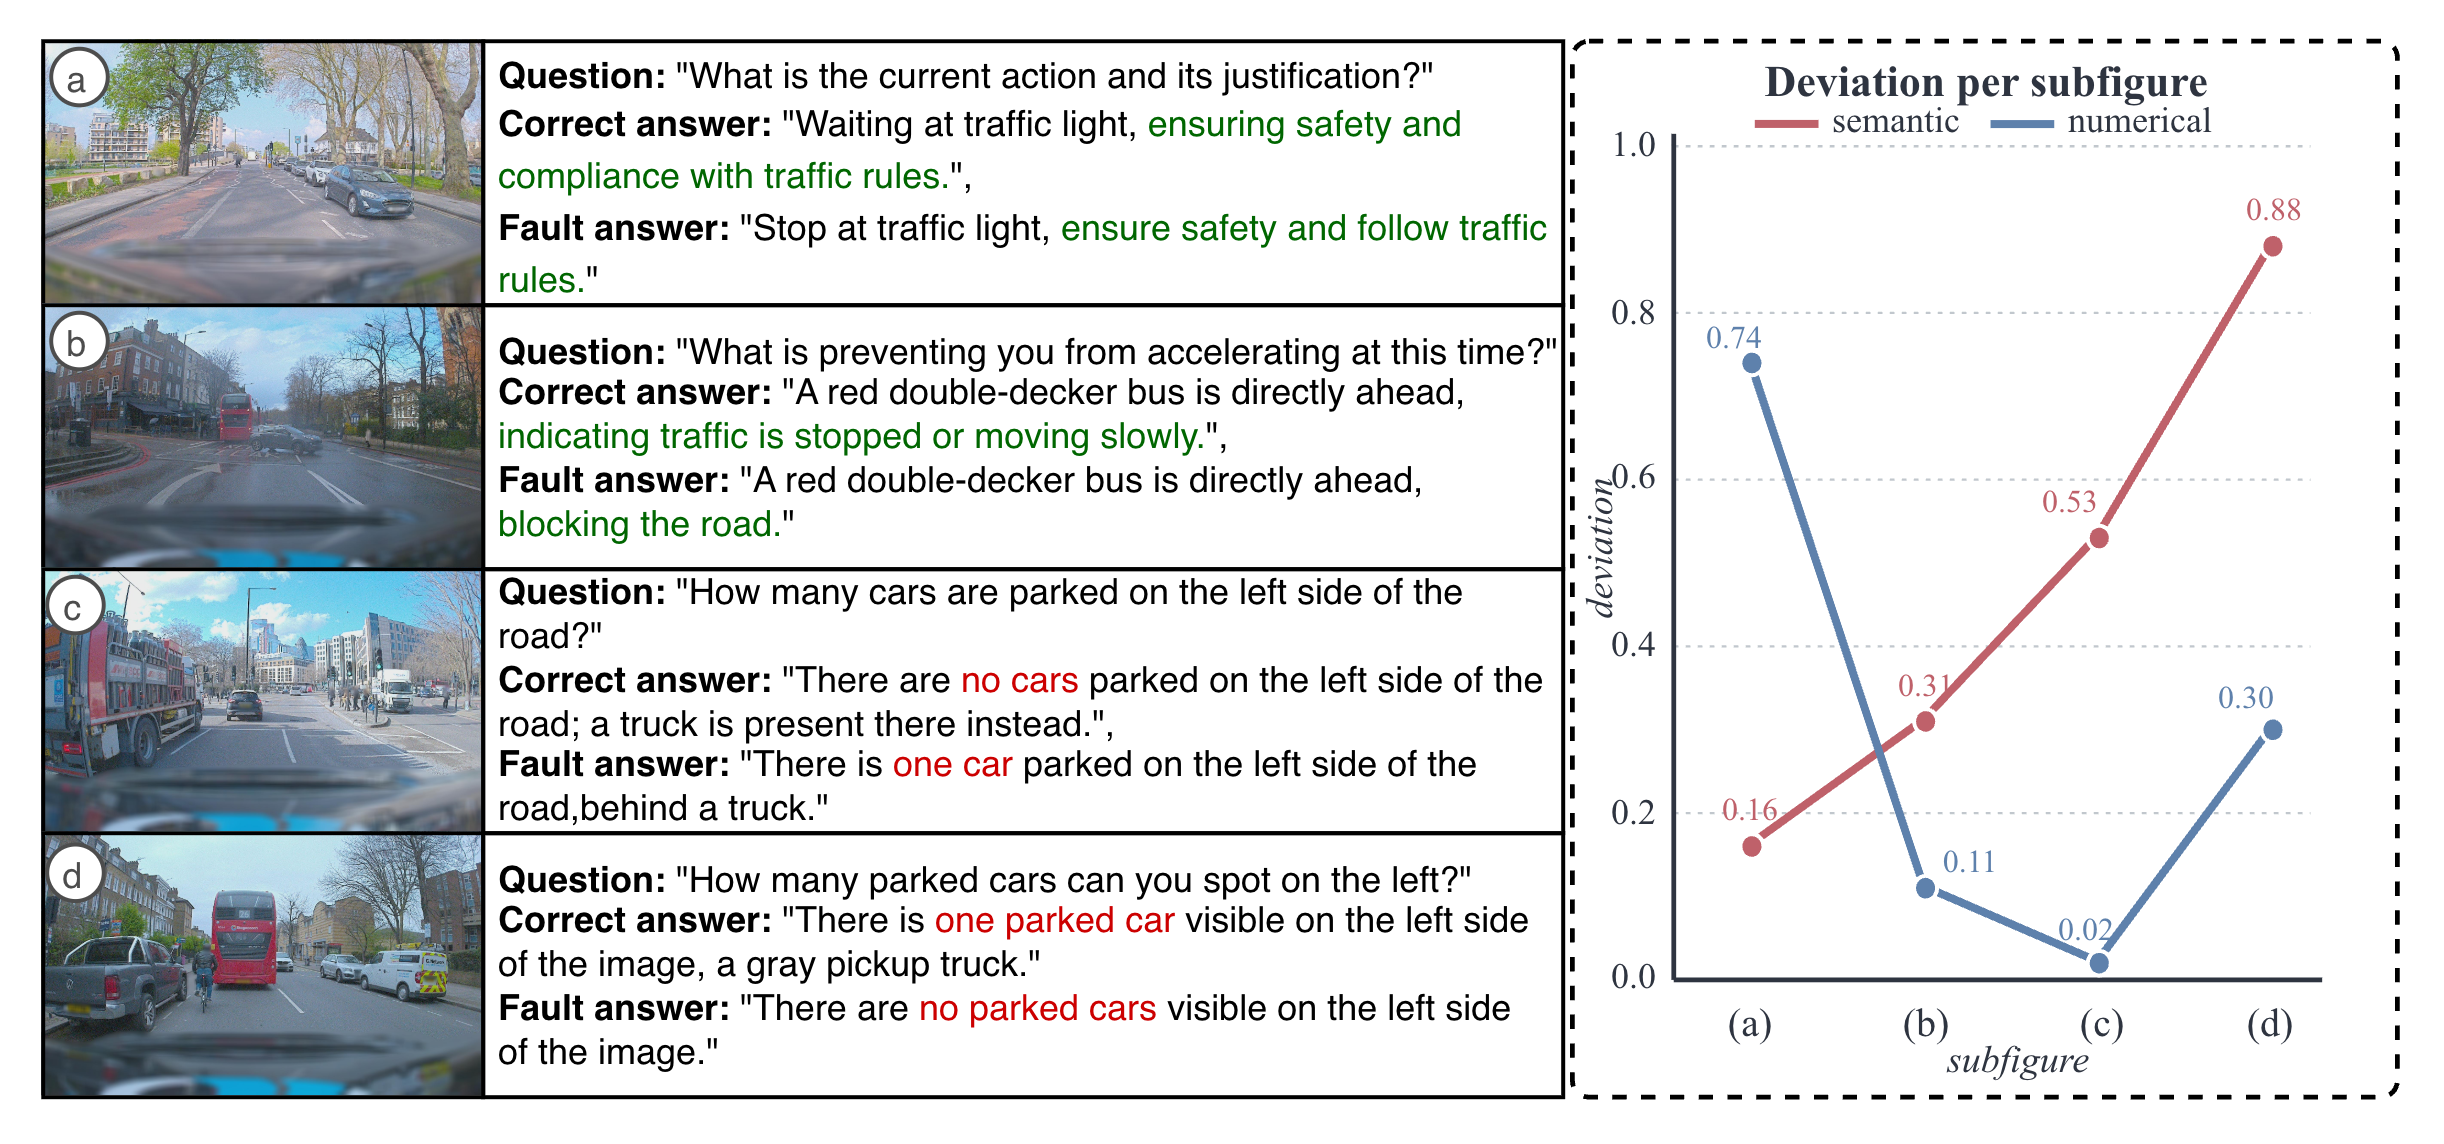
\includegraphics[width=1.0\linewidth]{Figures/figure1_examples_of_SDC_outputs.png}
    \caption{Examples of SDC outputs with different numerical and semantic deviations. The line chart (right) plots the two deviation types per subfigure, showing they do not correspond.}
    \label{fig:1}
\end{figure}

Existing soft error detection methods, such as Ranger and Dr.DNA, typically assess fault impact based on the activation range or numerical distribution. However, as the line chart in Figure~\ref{fig:1} illustrates, there is no one-to-one correspondence between the numerical deviation and the semantic deviation of the output in LLMs: a large numerical perturbation may be absorbed by subsequent computation, while a small one may propagate through the network and alter key generated content. Methods with fixed numerical thresholds therefore tend to suffer from both missed Significant SDCs and false alarms on non-critical faults. An effective detector must further characterize how faults affect the semantic representations inside the model.

We propose \textbf{SIEVE}, a lightweight, semantics-aware soft error detection framework for LLMs. SIEVE monitors selected adjacent decoder layers during inference, projects their intermediate representations into a low-dimensional space, and uses a Nominal Inter-Layer Predictor trained on clean execution traces to model the nominal inter-layer mapping. At runtime, the deviation of the actual representations from this mapping is aggregated into a layer-wise \textbf{Discrepancy Profile}; after further aggregation over multiple decoding steps, an independently calibrated lightweight classifier judges whether the current execution suffers a Significant SDC.

We systematically evaluate SIEVE on three representative LLMs and three VQA datasets. Under an evaluation protocol with semantically isolated splits and frozen thresholds (\S\ref{sec:experiments}), SIEVE achieves a macro-average F1 of 93.78\% and a non-Significant-SDC false positive rate of 0.107\% on the Test set of the nine tasks, with an end-to-end overhead of about 6.65\%, substantially outperforming the Ranger and Dr.DNA baselines under identical configurations.

Our main contributions are summarized as follows:
\begin{itemize}
  \item We formulate the Significant SDC problem for LLM inference, and reveal through systematic fault injection the inconsistency between the magnitude of numerical anomalies and the final semantic damage, thereby arguing the inherent limitations of the numerical-threshold detection paradigm.
  \item We propose SIEVE, a lightweight online Significant SDC detection framework. SIEVE learns the nominal transformation of representations between adjacent layers from clean traces, and constructs a Discrepancy Profile from the deviation between predicted and actual representations as the detection signal for Significant SDCs, which a lightweight classifier then judges.
  \item We conduct a unified evaluation on three LLMs and three VQA datasets. Under the best configuration, SIEVE achieves a macro-average F1 of 93.78\%, a recall of 91.49\%, and an FPR of 0.107\% on the Test set, improving over same-configuration baselines by up to 11.38 percentage points.
\end{itemize}

\section{Design Motivation}
\label{sec:motivation}

\subsection{Focus on Significant SDCs}
\label{sec:motivation-target}
\begin{wrapfigure}{r}{0.42\textwidth}
  \centering
  \vspace{-10pt}
  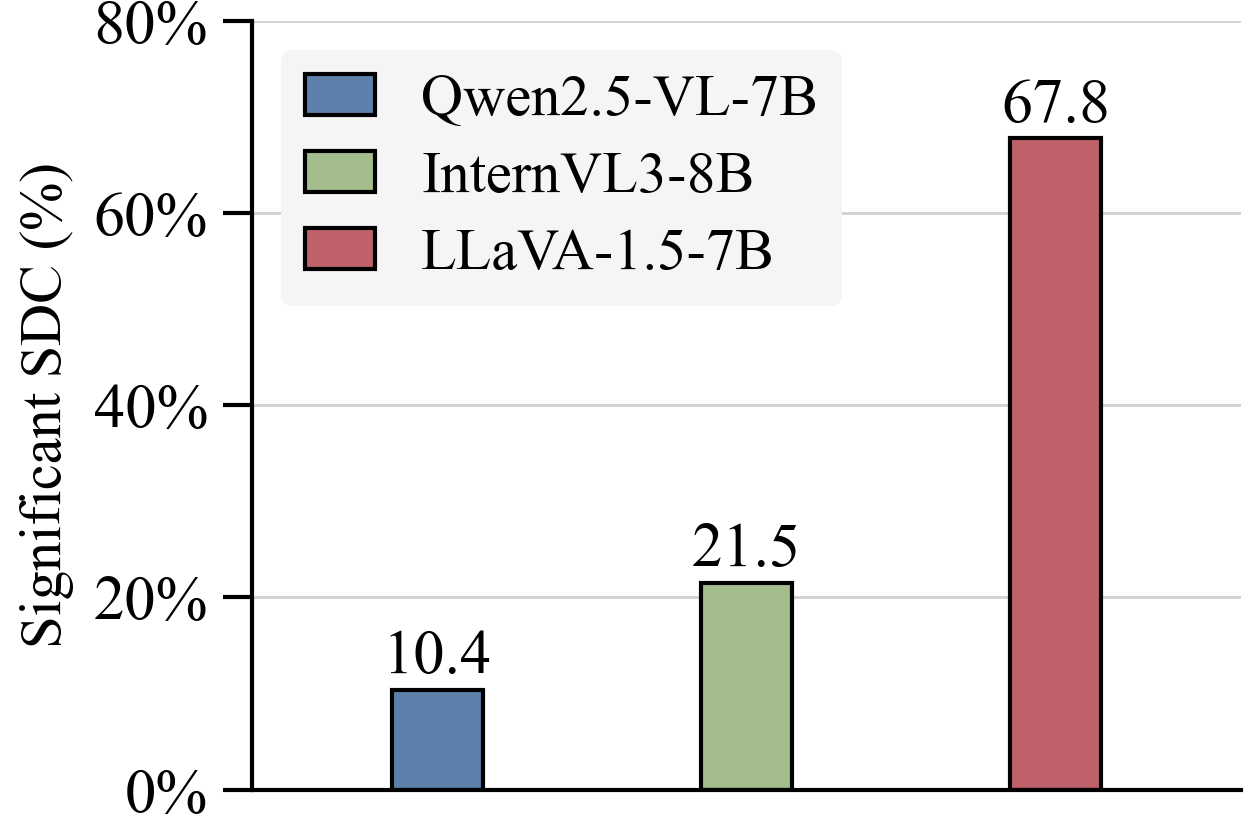
\includegraphics[width=\linewidth]{Figures/figure2_significant_SDC_share.png}
  \caption{Mean fraction of Significant SDCs among all SDCs.}
  \label{fig:2}
  \vspace{-10pt}
\end{wrapfigure}
The inherent fault tolerance of models creates a fault-masking effect that substantially raises the difficulty of SDC detection: not every hardware fault that triggers an SDC leads to catastrophic consequences. Following the definition in \S\ref{sec:intro}, an execution is marked as a \textit{Significant SDC} when its faulty output deviates from the normal output and the evaluation by an LLM-as-a-Judge (supplemented by manual review) identifies semantic deviations such as severe factual errors. As shown in Figure~\ref{fig:2}, when averaged over the three datasets, Significant SDCs account for 10.4\%, 21.5\%, and 67.8\% of all SDCs for Qwen2.5-VL-7B, InternVL3-8B, and LLaVA-1.5-7B, respectively. This indicates that most SDCs have limited semantic impact. detection should therefore focus on the small subset of Significant SDCs with severe consequences, which also reduces the number of detection targets and the subsequent error-recovery cost.

\subsection{Limitations of Numerical Deviation Detection}
\label{sec:motivation-numerical}
\begin{wrapfigure}{r}{0.42\textwidth}
  \centering
  \vspace{-10pt}
  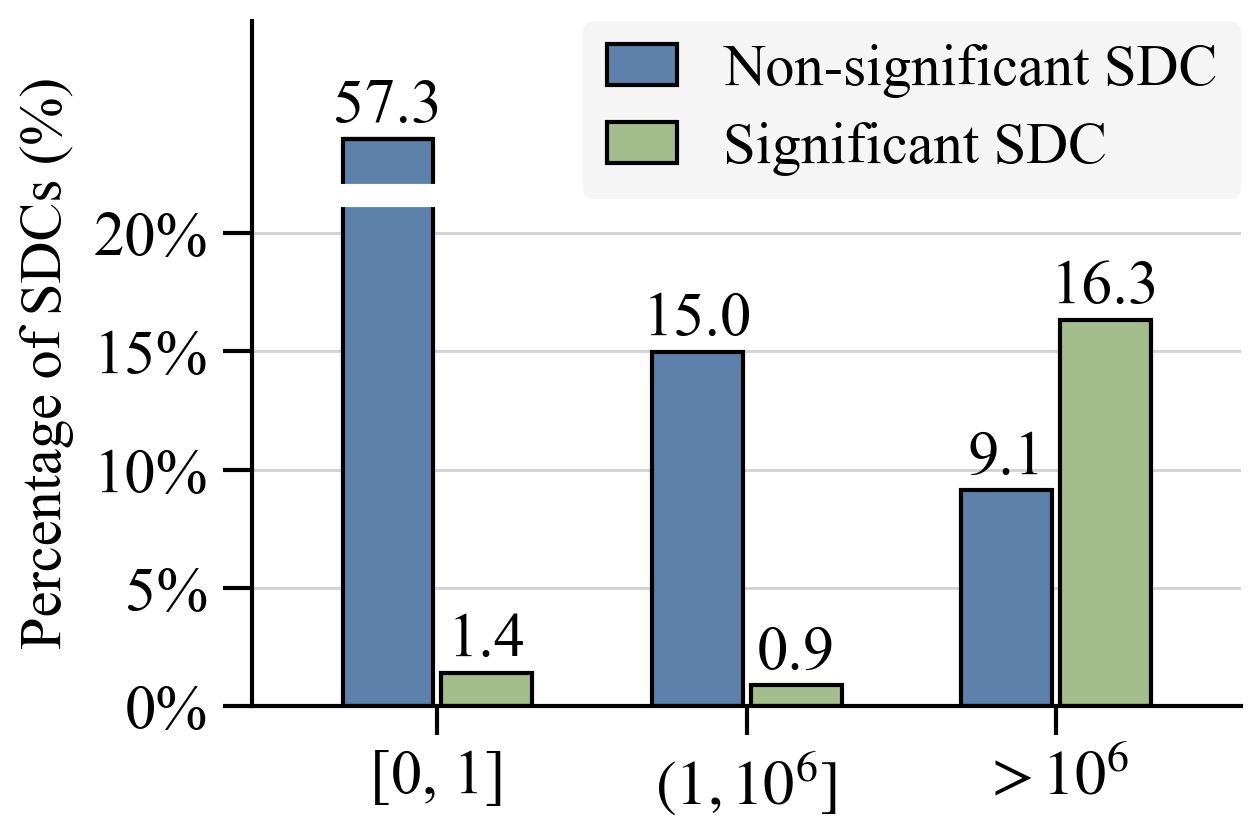
\includegraphics[width=\linewidth]{Figures/figure3_distribution_of_SDCs_by_numerical_deviation.png}
  \caption{Distribution of Non-Significant SDCs and Significant SDCs across three fault-induced value-deviation bins for finite-value faults.}
  \label{fig:3}
  \vspace{-10pt}
\end{wrapfigure}

Existing soft error detection methods typically judge fault impact by whether activations exceed normal ranges or deviate from normal distributions, implicitly assuming that a larger numerical deviation corresponds to a more severe impact. However, in LLMs, numerical deviation and output semantic damage are correlated yet not equivalent. Figure~\ref{fig:3} analyzes only faults whose injected scalar remains finite before and after the fault, and bins them by numerical deviation magnitude into three intervals: Significant SDCs already exist in the low-deviation interval, while in the high-deviation interval most faults cause no significant semantic damage. Detecting with a fixed threshold (e.g., 1) would miss 1.4\% of the Significant SDCs and raise unnecessary alarms for 24.1\% of the non-significant SDCs. Therefore, Significant SDC detection cannot rely on the magnitude of numerical deviation itself, but must characterize how faults affect the model's internal features.


\section{SIEVE Design}
\subsection{Overview}
The overall framework of SIEVE consists of three stages, as illustrated in Figure~\ref{fig:4}.

\textbf{Stage I}: Nominal Inter-Layer Predictor Training. At each decoding step, SIEVE collects the last-token representation of the self-attention output projection (\texttt{o\_proj}) from the monitored decoder layers and reduces it to a low-dimensional space with a shared random orthogonal matrix. A layer-aware predictor is then trained on clean execution traces to learn the nominal mapping between adjacent monitored layers, providing a per-step runtime reference for subsequent discrepancy computation.

\textbf{Stage II}: Significant SDC Detector Training. Under fault injection configurations, the predictor trained in Stage I estimates the nominal downstream representation for each selected layer pair, which is paired with the actually observed representation during faulty execution. Over the first $K$ decoding steps, the cosine similarity, signed mean and standard-deviation differences, and L2 distance between the predicted and observed representations are aggregated into a Discrepancy Profile. Combined with semantic severity labels generated by an LLM Judge, these profiles are used to train a lightweight XGBoost detector that identifies SDCs significantly impacting the semantic output of the model.

\textbf{Stage III}: Online Significant SDC Detection. During actual deployment, only the trained Nominal Inter-Layer Predictor and the XGBoost detector are executed online, performing real-time Significant SDC detection from runtime intermediate features. Since the entire detection process requires neither additional fault-free inference nor substantial computational complexity, it effectively reduces runtime overhead while maintaining detection capability.

\begin{figure}[!ht]
\centering
    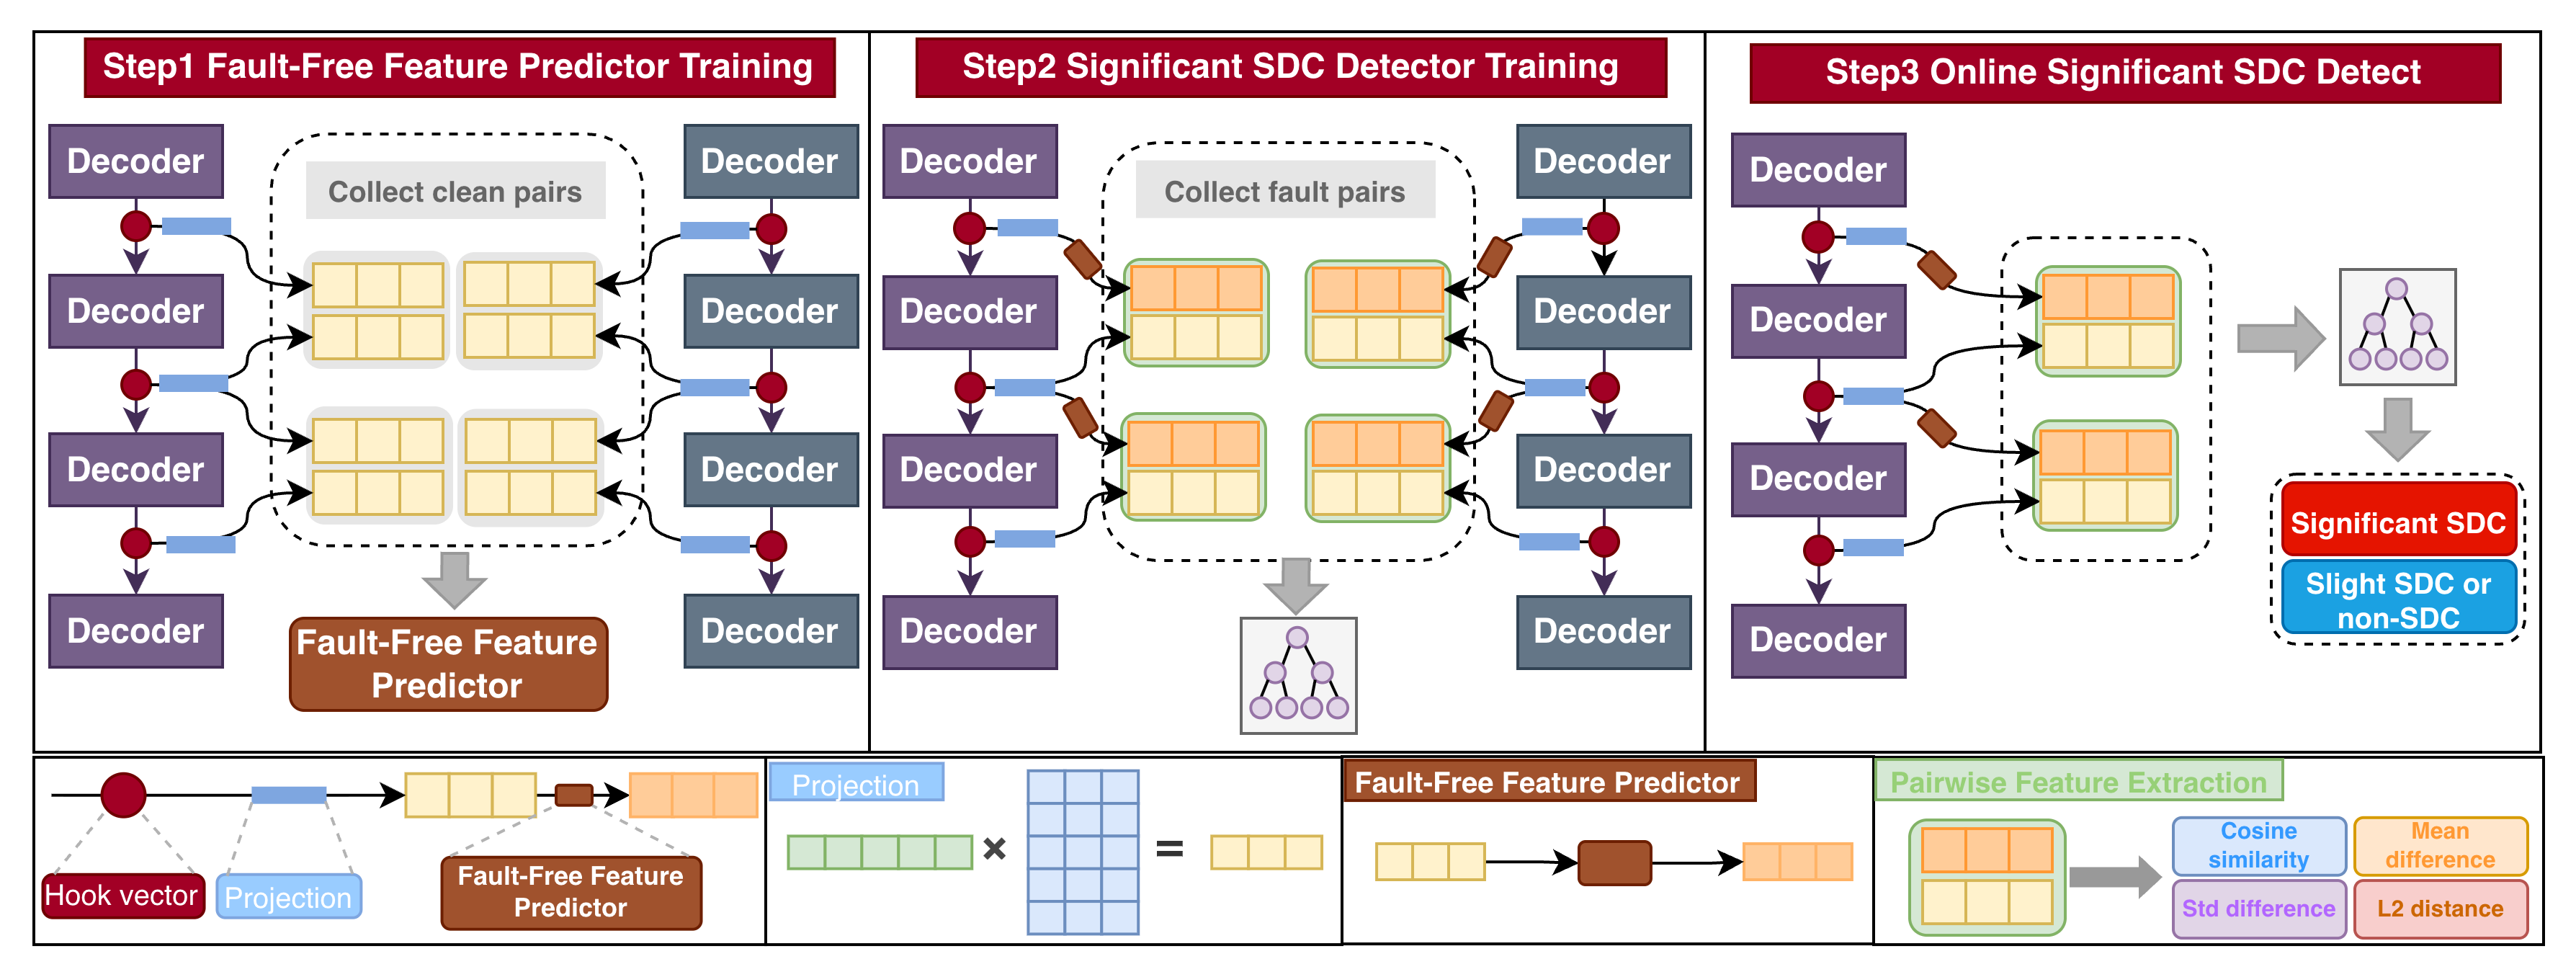
\includegraphics[width=1.0\linewidth]{Figures/figure4_SIEVE_overview.png}
    \caption{Overview of SIEVE. Per-layer attention outputs are projected to a low-dimensional space, a Nominal Inter-Layer Predictor models the nominal mapping between adjacent layers, and the resulting Discrepancy Profile feeds an XGBoost detector to flag Significant SDCs.}
    \label{fig:4}
\end{figure}

\subsection{Nominal Inter-Layer Predictor}
\subsubsection{Feature Collection}
To establish comparable reference features for runtime detection, we leverage PyTorch forward hooks to collect, at each decoding step of clean execution, the last-token representation of the self-attention output projection (\texttt{o\_proj}) of each monitored decoder layer, and organize adjacent monitored layers into feature pairs: the source-layer representation serves as the predictor's input while the target-layer representation acts as the supervision signal, learning the nominal inter-layer feature mapping. However, raw decoder features are extremely high-dimensional (e.g., 3,584 for Qwen2.5-VL-7B), making direct storage and training costly and increasing the difficulty of learning the mapping.

To this end, we project the features into a low-dimensional space. This design is inspired by the Johnson–Lindenstrauss (JL) lemma~\cite{johnson1984extensions}—random low-dimensional projections approximately preserve the geometric relations among samples—and employs a shared column-orthogonal projection matrix that maps features into a 64-dimensional space. Figure~\ref{fig:jl} (appendix) verifies this empirically via heatmaps of adjacent-layer relations and correlation scatter plots before and after projection: the reduced representations remain highly consistent with the original space, with Pearson and Spearman correlations of 0.909 and 0.902. The 64-dimensional projection thus preserves the dominant cross-layer geometric structure while substantially reducing both feature storage and predictor size.


\subsubsection{Predictor Training}
The predictor is trained to reconstruct the nominal feature of a target layer from the low-dimensional feature of its source layer. Since intermediate features require both element-wise numerical accuracy and the semantic consistency carried by their direction, supervising with Mean Squared Error (MSE) alone biases the model toward element-wise fidelity at the expense of directional consistency. We therefore adopt a combined objective. Let $\hat{\mathbf{Y}}$ denote the predictor's output and $\mathbf{Y}$ the corresponding nominal target feature; the training loss is
$$L = \alpha L_{\mathrm{mse}} + \beta L_{\mathrm{cos}}, \qquad L_{\mathrm{cos}} = 1 - \cos(\hat{\mathbf{Y}}, \mathbf{Y}),$$
where $\alpha$ and $\beta$ are hyperparameters that balance the two loss terms, both set to 1.0 in this work. The MSE term ensures numerical fidelity, while the cosine term constrains directional consistency in the representation space, yielding stable and semantically coherent predictions. Architecturally, the predictor is a layer-aware residual MLP: each 64-dimensional source feature is concatenated with a 16-dimensional layer embedding and passed through 8 residual blocks (hidden size 64, dropout 0.1) to produce the 64-dimensional nominal feature of the target layer, allowing a single shared network to distinguish the mapping of each monitored layer pair. After training, the predictor performs only one lightweight forward pass per step at runtime, and its output serves as the reference for the subsequent Discrepancy Profile.

\subsection{Significant SDC Detector Training}

\subsubsection{Discrepancy Profile}
To capture Significant-SDC signatures from the nominal reference features provided by the predictor, we construct a Discrepancy Profile that characterizes each predicted--actual feature pair from two perspectives: (1) \emph{statistical discrepancy}---the signed differences of mean and standard deviation, capturing global numerical shifts with their direction and changes in dispersion; and (2) \emph{geometric discrepancy}---the cosine similarity and L2 distance, capturing directional consistency and absolute deviation magnitude. Each layer pair thus yields a four-dimensional discrepancy vector, which we aggregate over the first $K$ decoding steps into the mean, maximum, and minimum of every metric and concatenate in a fixed order, giving a fixed 12-dimensional feature vector per pair; a configuration that monitors $P$ layer pairs therefore presents a $12P$-dimensional input to the Detector.

\subsubsection{Detector Dataset Construction}

Training data is produced by the fault injection experiments: for each faulty execution, the Discrepancy Profiles extracted from all monitored layer pairs form one training sample, which consists solely of low-dimensional statistical and geometric metrics and is therefore compact and easy to train on.

Semantic labels are generated by Prometheus-7B as the LLM Judge, which receives the original task instruction, the faulty output, and the fault-free baseline output, and scores the pair with a fixed three-level rubric: 2 for semantic equivalence, 1 for slight deviation with the core answer largely preserved, and 0 for a changed, missing, or contradictory core answer. A score of 0 is labeled Significant SDC and 1/2 as Slight/Non-SDC. The label measures the incremental semantic impact of the fault relative to fault-free execution, not whether the model's answer is correct; all samples are manually re-reviewed, and a unified system prompt, template, and rubric are used to ensure reproducibility.

\subsubsection{Significant SDC Detector}
We adopt XGBoost as the detector: the 36-dimensional feature space is small, gradient-boosted trees efficiently model nonlinear interactions within it, and tree inference is far cheaper than a deep network, suiting online detection. After training, the Detector directly consumes the Discrepancy Profile and outputs the Significant SDC probability and binary decision, providing the basis for subsequent error recovery. Through this process, SIEVE reduces semantic error detection to a supervised classification problem over low-dimensional features, maintaining accuracy while keeping runtime overhead low.

\subsection{Online Detection Workflow}
During online deployment, SIEVE performs no training or parameter updates and attaches to the LLM in a read-only bypass via PyTorch Forward Hooks, leaving activations and generation logic unmodified. At each decoding step, the last-token \texttt{o\_proj} features of the monitored layers are projected into a shared 64-dimensional space by a fixed column-orthogonal matrix; each pair's Nominal Inter-Layer Predictor estimates the target layer's nominal feature from the source layer, and the predicted--actual comparison forms the Discrepancy Profile. SIEVE then aggregates features once over the first $K=\min(28,T)$ decoding steps; if EOS occurs earlier, all available steps are used, preserving coverage for short outputs. For each pair, the mean, maximum, and minimum of the four metrics are concatenated into the 36-dimensional Discrepancy Profile, which the XGBoost Detector maps to a Significant-SDC probability and binary decision.

\section{Experiments}
\label{sec:experiments}
\subsection{Experimental Setup}
\label{sec:setup}

\paragraph{Models, datasets, and splits.}
We evaluate SIEVE on Qwen2.5-VL-7B \cite{Qwen2VL}, InternVL3-8B \cite{chen2024internvl}, and LLaVA-1.5-7B \cite{liu2023visual} using EarthVQA \cite{wang2024earthvqa}, LingoQA \cite{marcu2024lingoqa}, and VQAv2 \cite{balanced_vqa_v2}, yielding nine model--dataset tasks. Each task targets 5{,}000 fault-free executions and 50{,}000 random dual-bit fault injections; valid-execution counts are reported in Table~\ref{tab:A1} (appendix). Executions sharing the same image or question are assigned as a whole to disjoint Training / Validation / Test partitions (70\% / 15\% / 15\%). Faulty Training records train the Detector; fault-free telemetry within Training is further split into predictor fit / early-stopping / evaluation subsets under the same group rule. Validation freezes thresholds; Test is used only for final scoring.

\paragraph{Fault injection.}
We emulate transient soft errors by software fault injection: during prefill, we randomly select a \texttt{torch.nn.Linear} module and flip two random bits of a random scalar in its output tensor. Only executions that complete normally and yield extractable features are counted. Each faulty output is labeled Non-SDC, Non-significant SDC, or Significant SDC by an LLM judge, from its semantic change relative to the fault-free baseline on the same input.

\subsection{SDC Detector Evaluation}

\subsubsection{Detection Performance}
We perform nested selection over 40 feature-dimension/window combinations within the outer Training set only, ultimately adopting 36D with $K=28$: monitored pairs $(6,7)$, $(24,25)$, and $(26,27)$, aggregated over the first $\min(28,T)$ actual decoding steps (Appendix~\ref{app:config}). Neither Ranger nor Dr.DNA provides a public implementation, so we re-implement their detection mechanisms following the original papers to ensure a fair comparison under identical configurations, rather than claiming to reproduce the complete original systems. Concretely, all three methods share the same monitored layers, decoding steps, fault instances, and outer data partitions, and each freezes its threshold on the Validation set only; clean reference profiles for Ranger and Dr.DNA are built from a 20\% group subset determined in the Training set, with remaining details in Table~\ref{tab:A2}. During evaluation, all methods are scored on exactly the same executions, matched row-by-row by sample identity, output, and fault metadata, with effective coverage in Table~\ref{tab:A1}. Each task's XGBoost Detector is trained on the Training set, and its threshold is chosen on the Validation set to maximize Significant-SDC F1. As shown in Table~\ref{tab:det_no_filter}, on the Test set SIEVE improves the nine-task average F1 over Ranger and Dr.DNA by 10.33 and 11.38 percentage points.
\begin{table}[!ht]
  \centering
  \caption{Per-task Significant-SDC detection results on the Test set (\%); P/R/F1 denote Precision/Recall/F1.}
  \label{tab:det_no_filter}
  \footnotesize
  \setlength{\tabcolsep}{4pt}
  \renewcommand{\arraystretch}{1.05}
  \resizebox{\linewidth}{!}{%
  \begin{tabular}{llccccccccc}
  \toprule
  & & \multicolumn{3}{c}{\textbf{EarthVQA}} & \multicolumn{3}{c}{\textbf{LingoQA}} & \multicolumn{3}{c}{\textbf{VQAv2}} \\
  \cmidrule(lr){3-5} \cmidrule(lr){6-8} \cmidrule(lr){9-11}
  \textbf{Model} & \textbf{Method} & \textbf{P} & \textbf{R} & \textbf{F1} & \textbf{P} & \textbf{R} & \textbf{F1} & \textbf{P} & \textbf{R} & \textbf{F1} \\
  \midrule
  \multirow{3}{*}{Qwen2.5-VL-7B}
   & Ranger & 94.85  & 81.85 & 87.87 & 49.87  & 92.92 & 64.91 & 63.02  & 81.61 & 71.12 \\
   & Dr.DNA & 100.00 & 61.48 & 76.15 & 52.33  & 74.06 & 61.33 & 79.71  & 63.22 & 70.51 \\
   & SIEVE  & 89.54  & 85.56 & 87.50 & 99.49  & 92.93 & 96.10 & 100.00 & 84.29 & 91.48 \\
  \cmidrule(lr){2-11}
  \multirow{3}{*}{InternVL3-8B}
   & Ranger & 85.77  & 95.76 & 90.49 & 66.22  & 89.54 & 76.13 & 94.57  & 72.76 & 82.25 \\
   & Dr.DNA & 97.63  & 78.39 & 86.96 & 99.43  & 70.02 & 82.17 & 99.12  & 67.00 & 79.95 \\
   & SIEVE  & 99.57  & 97.67 & 98.61 & 99.35  & 91.75 & 95.40 & 97.06  & 91.85 & 94.38 \\
  \cmidrule(lr){2-11}
  \multirow{3}{*}{LLaVA-1.5-7B}
   & Ranger & 86.67  & 95.97 & 91.08 & 100.00 & 85.03 & 91.91 & 100.00 & 91.12 & 95.36 \\
   & Dr.DNA & 100.00 & 95.97 & 97.95 & 100.00 & 85.56 & 92.22 & 100.00 & 89.35 & 94.38 \\
   & SIEVE  & 95.36  & 96.64 & 96.00 & 99.41  & 90.37 & 94.68 & 87.64  & 92.31 & 89.91 \\
  \midrule
  \multirow{3}{*}{Average}
   & Ranger & 89.10 & 91.19 & 89.81 & 72.03 & 89.16 & 77.65 & 85.86 & 81.83 & 82.91 \\
   & Dr.DNA & 99.21 & 78.61 & 87.02 & 83.92 & 76.55 & 78.57 & 92.94 & 73.19 & 81.61 \\
   & \textbf{SIEVE} & \textbf{94.82} & \textbf{93.29} & \textbf{94.04} & \textbf{99.42} & \textbf{91.68} & \textbf{95.39} & \textbf{94.90} & \textbf{89.48} & \textbf{91.92} \\
  \bottomrule
  \end{tabular}%
  }
\end{table}

Some executions produce NaN or $\pm\mathrm{Inf}$ values among the monitored features after injection, and such extreme values are trivially detected by any method. To verify whether the methods genuinely distinguish the harder cases, we filter out these executions and re-score all three methods on the remaining ones whose 36 features are all finite, with no retraining or recalibration; Table~\ref{tab:det_finite} reports the result. The average F1 of Ranger and Dr.DNA drops from 83.46 and 82.40 in Table~\ref{tab:det_no_filter} to 37.74 and 22.74, whereas SIEVE degrades far less (93.78 to 68.78) and exceeds both baselines by a wide margin on most tasks, attaining the highest F1 on seven of the nine. Its advantage therefore comes from discriminating genuinely ambiguous finite-value faults rather than from obvious non-finite signals.

\begin{table}[!ht]
  \centering
  \caption{Per-task Significant-SDC detection on the Test set after excluding executions with non-finite features (\%).}
  \label{tab:det_finite}
  \footnotesize
  \setlength{\tabcolsep}{4pt}
  \renewcommand{\arraystretch}{1.05}
  \resizebox{\linewidth}{!}{%
  \begin{tabular}{llccccccccc}
  \toprule
  & & \multicolumn{3}{c}{\textbf{EarthVQA}} & \multicolumn{3}{c}{\textbf{LingoQA}} & \multicolumn{3}{c}{\textbf{VQAv2}} \\
  \cmidrule(lr){3-5} \cmidrule(lr){6-8} \cmidrule(lr){9-11}
  \textbf{Model} & \textbf{Method} & \textbf{P} & \textbf{R} & \textbf{F1} & \textbf{P} & \textbf{R} & \textbf{F1} & \textbf{P} & \textbf{R} & \textbf{F1} \\
  \midrule
  \multirow{3}{*}{Qwen2.5-VL-7B}
   & Ranger & 83.78  & 55.86 & 67.03 & 20.80  & 77.61 & 32.81 & 27.75  & 50.00 & 35.69 \\
   & Dr.DNA & 100.00 & 18.92 & 31.82 & 11.18  & 26.87 & 15.79 & 8.70   & 4.17  & 5.63 \\
   & SIEVE  & 72.73  & 64.86 & 68.57 & 98.11  & 77.61 & 86.67 & 100.00 & 57.29 & 72.85 \\
  \cmidrule(lr){2-11}
  \multirow{3}{*}{InternVL3-8B}
   & Ranger & 58.56  & 84.13 & 69.06 & 30.37  & 65.56 & 41.51 & 60.38  & 18.93 & 28.83 \\
   & Dr.DNA & 79.07  & 26.98 & 40.24 & 85.71  & 7.95  & 14.55 & 80.00  & 7.10  & 13.04 \\
   & SIEVE  & 98.29  & 91.27 & 94.65 & 97.35  & 72.85 & 83.33 & 90.14  & 75.74 & 82.32 \\
  \cmidrule(lr){2-11}
  \multirow{3}{*}{LLaVA-1.5-7B}
   & Ranger & 21.43  & 50.00 & 30.00 & 0.00   & 0.00  & 0.00  & 100.00 & 21.05 & 34.78 \\
   & Dr.DNA & 100.00 & 50.00 & 66.67 & 100.00 & 3.57  & 6.90  & 100.00 & 5.26  & 10.00 \\
   & SIEVE  & 50.00  & 58.33 & 53.85 & 90.91  & 35.71 & 51.28 & 21.43  & 31.58 & 25.53 \\
  \midrule
  \multirow{3}{*}{Average}
   & Ranger & 54.59 & 63.33 & 55.36 & 17.06 & 47.72 & 24.77 & 62.71 & 29.99 & 33.10 \\
   & Dr.DNA & 93.02 & 31.97 & 46.24 & 65.63 & 12.80 & 12.41 & 62.90 & 5.51  & 9.56 \\
   & \textbf{SIEVE} & \textbf{73.67} & \textbf{71.49} & \textbf{72.36} & \textbf{95.46} & \textbf{62.06} & \textbf{73.76} & \textbf{70.52} & \textbf{54.87} & \textbf{60.23} \\
  \bottomrule
  \end{tabular}%
  }
\end{table}

\subsubsection{Detection Overhead}
\begin{wraptable}{l}{3.1in}
  \vspace{-12pt}
  \refstepcounter{table}%
  {\raggedright Table~\thetable: End-to-end mean latency and relative overhead (\%) on LingoQA.\par}
  \label{tab:sieve_online_overhead}
  \vspace{2pt}
  \small
  \resizebox{2.95in}{!}{%
  \begin{tabular}{lcccc}
    \toprule
    Model & Baseline & Ranger & Dr.DNA & SIEVE \\
    \midrule
    Qwen2.5-VL-7B   & 764.4 & +1.77 & +3.82 & +6.44 \\
    InternVL3-8B    & 984.3 & +1.78 & +5.20 & +6.53 \\
    LLaVA-1.5-7B    & 363.8 & +2.75 & +5.67 & +6.98 \\
    \bottomrule
  \end{tabular}%
  }
\end{wraptable}
We measure end-to-end overhead on a single NVIDIA H20 GPU with batch size 1. All four detection modes use the same six monitored layers and run over the first $\min(28,T)$ actual decoding steps. Each model executes 10 warmup and 10 forward repetitions on 50 fixed LingoQA samples, yielding 500 observations per model--method pair. Answers under all monitored modes are identical to the baseline without detection. SIEVE's average overhead is 6.65\%, versus 2.10\% for Ranger and 4.89\% for Dr.DNA.

\subsection{Nominal Inter-Layer Predictor Evaluation}
As shown in Table~\ref{tab:fault_free_predictor_performance} (appendix), the trained Nominal Inter-Layer Predictor attains MSE from 0.0066 to 0.2207 and CosSim from 0.6367 to 0.9138 across the nine tasks; because activation scales differ across models, MSE is not comparable across models. We further examine how the prediction residual behaves under faults. Figure~\ref{fig:cosine-vis} shows the CosSim averaged over all actual decoding steps for each faulty run: Significant SDCs exhibit the lowest mean CosSim, while Non-SDC and Non-significant SDC overlap clearly, confirming that the predictor separates Significant SDCs from Non-significant SDCs well.

\begin{figure}[!ht]
\centering
    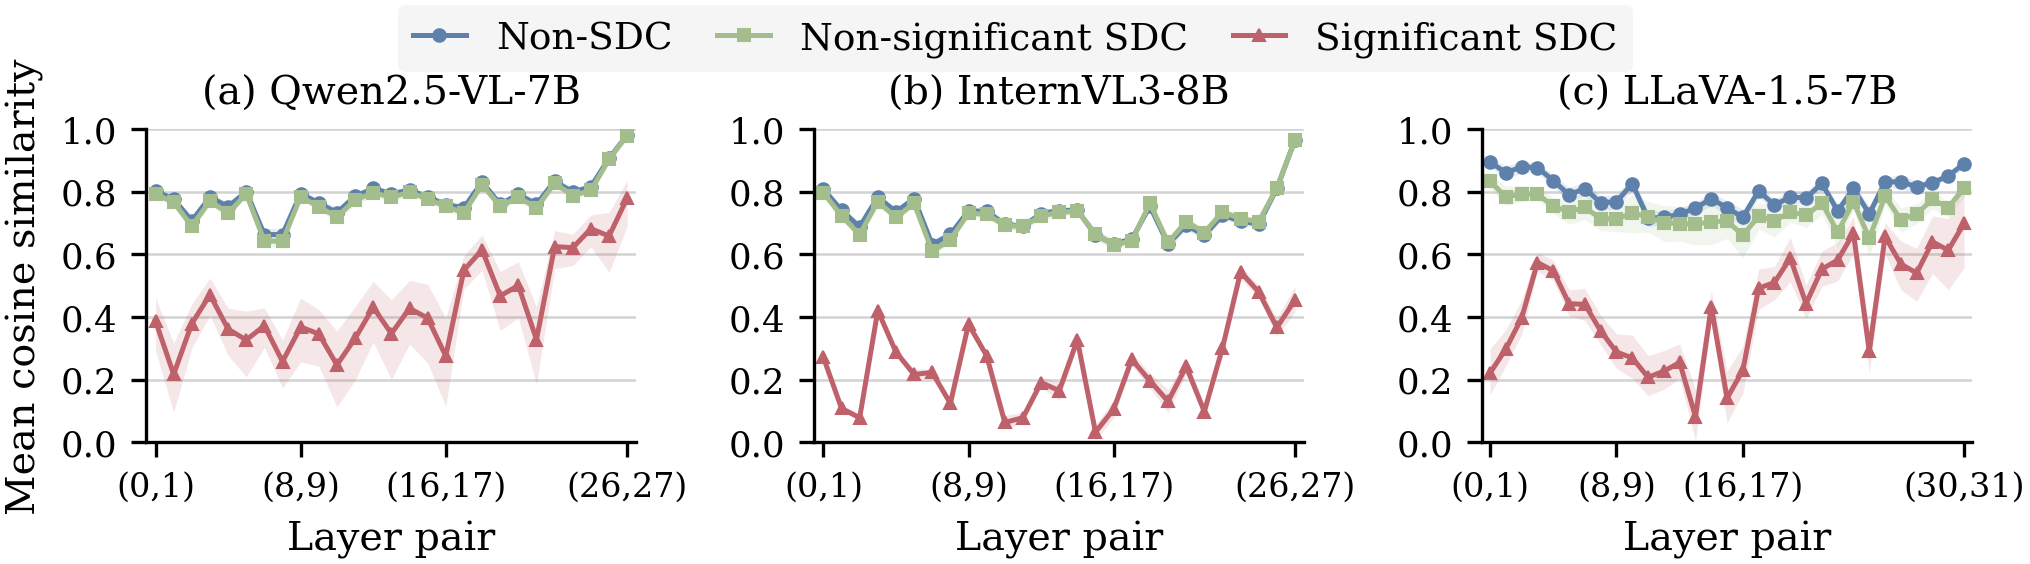
\includegraphics[width=1.0\linewidth]{Figures/figure6_layer_pair_cosine_similarity.png}
    \caption{Average finite CosSim per adjacent layer pair over actual decoding steps on LingoQA, grouped by execution category. Shaded bands are 95\% cluster bootstrap confidence intervals over images.}
    \label{fig:cosine-vis}
\end{figure}

\subsection{Ablation Study}
We ablate layer pairs and metrics at the fixed 36D/K=28 configuration. Layer-pair ablation removes all 12 features of one pair; metric ablation removes the 9 features of CosSim, Mean Difference, Std Difference, or L2 Distance across the three pairs. We additionally score only the executions whose 36 features are all finite, after the configuration has been frozen. As Figure~\ref{fig:ablation} shows, removing any component lowers the nine-task average Test F1. Removing $(26,27)$ and $(24,25)$ costs 2.47 and 2.16 F1 points, respectively; among metrics, Mean Difference is most critical ($-3.74$) and Std Difference contributes least ($-0.46$). The finite-value diagnostic shows the same overall trend. Complete per-task results on the Test set are in Table~\ref{tab:A5}, and those of the finite-value diagnostic are in Table~\ref{tab:A6} (appendix).

\begin{figure}[!ht]
\centering
    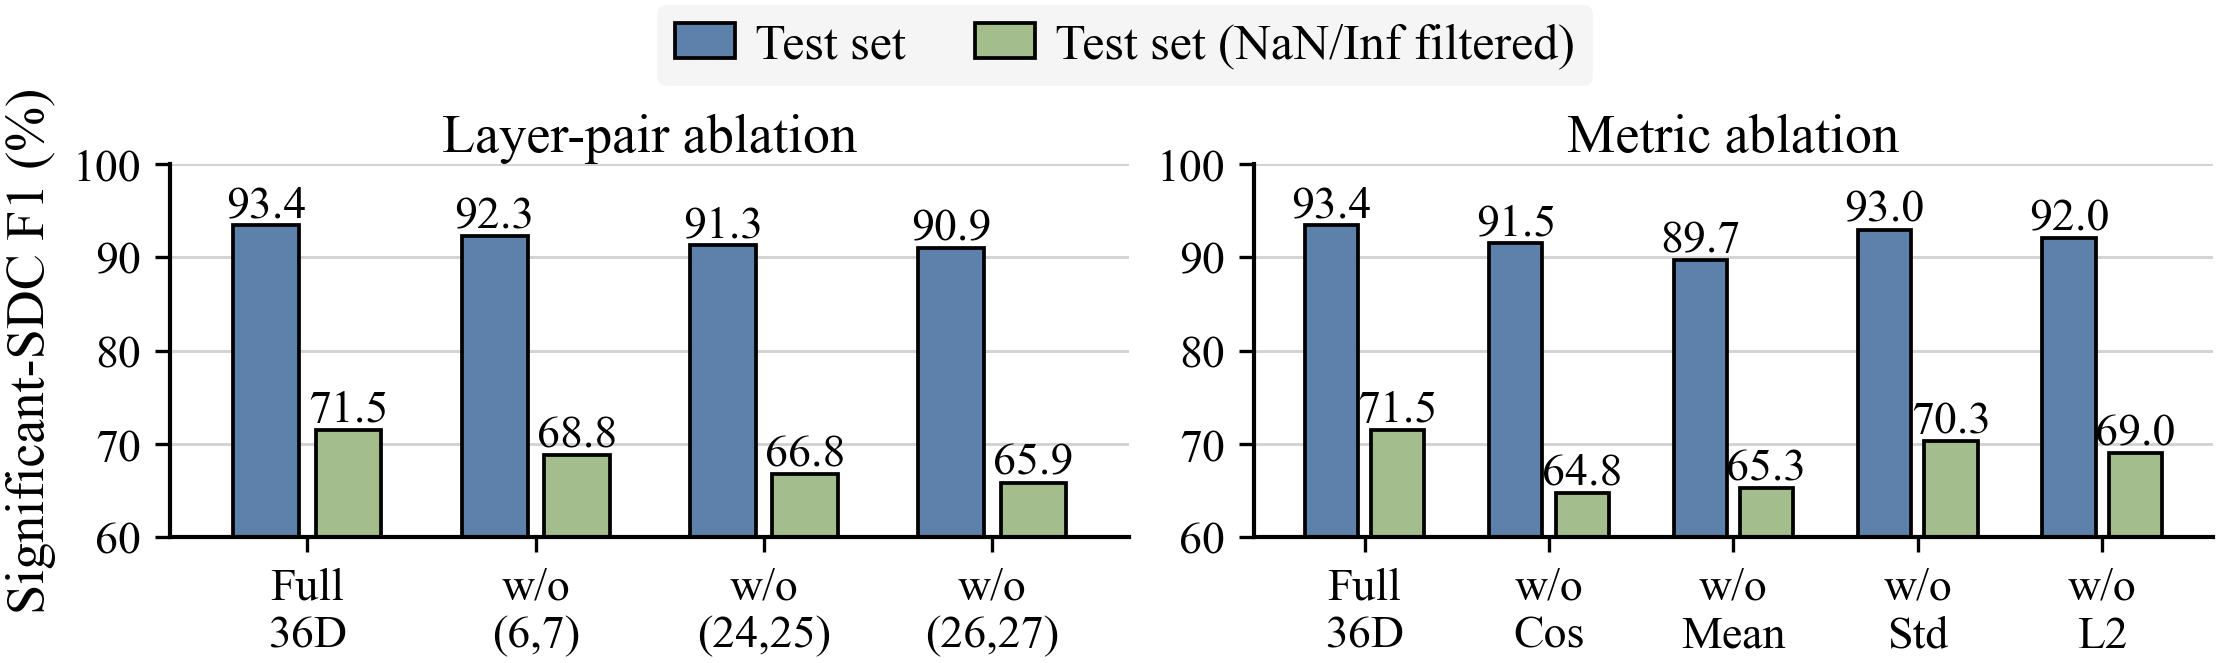
\includegraphics[width=1.0\linewidth]{Figures/figure7_component_ablation.png}
    \caption{Component ablation at 36D/K=28. Left: layer-pair ablation; right: metric ablation. Bars show nine-task average Significant-SDC F1.}
    \label{fig:ablation}
\end{figure}


\section{Related Work}
\label{sec:related}

\paragraph{Silent Data Corruption in Deep Learning Systems.}
Transient bit flips induced by cosmic rays, voltage noise, and device aging have long been studied as soft errors in digital microelectronics \cite{dodd2003basic}. As computational demand grows, such faults occur regularly in large GPU fleets and can silently corrupt results without raising any system exception \cite{wang2023understanding,wang2024understanding,he2023understanding,tan2025gerem}. For neural workloads, empirical studies further reveal that although most faults are naturally masked by the redundancy of activations and weights, a small fraction propagates into visibly wrong predictions \cite{xue2023soft,chen2025bit}; in LLM training, SDC events have been reported to disrupt large-scale runs \cite{ma2025understanding}. In LLM inference, a corrupted execution may surface as a fluent but semantically wrong answer, which is particularly dangerous in safety-critical deployments. These findings motivate a severity-aware view: the detection target should be the rare faults that materially change semantics, rather than all numerical deviations.

\paragraph{Fault Detection and Resilience Techniques for DNNs.}
Classical resilience mechanisms---ECC memory \cite{sullivan2023implicit}, triple modular redundancy \cite{mahmood2025design}, and GPU checkpoint/restore \cite{wei2025phoenixos,zeng2026gpu}---protect hardware uniformly and incur substantial performance or resource overhead at LLM scale. Lightweight alternatives exploit the error tolerance of neural networks themselves: algorithm-based fault tolerance embeds checksums or consistency constraints into linear layers and attention \cite{xue2023approxabft,liang2025attnchecker}; Ranger restricts activations to learned safe ranges to suppress fault propagation \cite{chen2021low}; Dr.DNA detects SDCs from deviations of neuron-activation distributions \cite{ma2024dr}; and structural hardening designs include fault-tolerant attention \cite{dai2025ft}, first-token-inspired online protection of critical layers \cite{sun2025ft2}, and sensitivity-guided selective protection \cite{xie2025realm}. All of these designs judge faults at the numerical or structural level, without asking whether a fault materially changes the generated semantics. As shown in \S\ref{sec:motivation-numerical}, the two views diverge for LLMs: semantic severity is not monotonic in numerical deviation.

\paragraph{Semantic Measures of Generated Text.}
A rich literature quantifies the semantic equivalence of texts. Embedding-based measures, such as BERT-based similarity \cite{devlin2019bert}, Sentence-BERT \cite{reimers2019sentence}, SimCSE \cite{gao2021simcse}, and the Universal Sentence Encoder \cite{cer2018universal}, compute similarity in a latent space and handle paraphrasing gracefully; cross-encoders jointly encode text pairs to capture finer-grained relations such as negation and entity mismatch \cite{nogueira2019passage,deshpande2023c,lin2025using}; and LLM-as-a-Judge protocols evaluate consistency against fixed rubrics with strong agreement with human judgment \cite{liu2023g,zheng2023judging}; this work therefore uses an LLM-as-a-Judge with a fixed rubric offline to define and label Significant SDCs (\S\ref{sec:motivation-target}).

\section{Conclusion}
\label{sec:conclusion}

This paper studied the semantic impact of soft errors in LLM inference. Numerical anomaly magnitude does not consistently track output severity, so detectors based on activation ranges or distribution shifts misjudge which faults matter. We proposed SIEVE, which models nominal inter-layer feature transitions from clean traces and judges Significant SDCs from the statistical and geometric discrepancy profile of prediction errors, without ground-truth answers or model modification. On three LLMs and three VQA datasets, SIEVE reaches a macro-average F1 of 93.78\% at an FPR of 0.11\% with 6.65\% end-to-end overhead, outperforming configuration-matched Ranger- and Dr.DNA baselines by more than 10 points. Scope limitations and future work are discussed in Appendix~\ref{app:limitations}.

\section*{AI use statement}

In this work, we used generative AI tools exclusively to assist with manuscript writing, including improving grammar and clarity and helping draft portions of the text, which we then rewrote and refined. We have not used generative AI tools for research ideation, for generating experiment code, or for analyzing results, and no other tasks requiring disclosure under the ICLR 2027 AI Policy for Authors are applicable to this work. All AI-assisted text was carefully reviewed by the authors for accuracy and originality. We take responsibility for the final content of this work, including text, claims, or artifacts produced with the aid of generative AI.

\section*{Ethics statement}

This work studies how to improve the reliability of large language model inference under hardware soft errors, with the goal of supporting safer deployment in safety-critical applications such as autonomous driving and remote sensing. We do not foresee any negative ethical consequences of our methods or findings. All experiments use publicly available models (Qwen2.5-VL, InternVL3, LLaVA) and publicly released VQA benchmarks (Appendix~\ref{app:dataset}); no human subjects were involved, no personal or user data were collected, and no new dataset is released. Severity labels are produced offline by an LLM-as-a-Judge protocol with a fixed rubric (\S\ref{sec:motivation-target}), which is used solely for evaluation and never as part of the deployed detector. The authors declare no competing interests and confirm that the research was conducted in compliance with the ICLR Code of Ethics.

\section*{Reproducibility statement}

To ensure reproducibility, we provide complete implementation details---model configurations, monitored layers, feature extraction, detector training, and evaluation protocols---in Appendix~\ref{app:impl}, the full configuration-selection procedure in Appendix~\ref{app:config}, and dataset and evaluation-scope statistics in Appendix~\ref{app:dataset}. The fault-injection and evaluation code, together with scripts to regenerate all figures and tables, is provided in an anonymized repository submitted as supplementary material.


\section*{Acknowledgments}
% Use unnumbered third level headings for the acknowledgments. All
% acknowledgments, including those to funding agencies, go at the end of the paper.


\bibliography{references}
\bibliographystyle{iclr2027_conference}

\appendix
\renewcommand{\thetable}{A\arabic{table}}
\setcounter{table}{0}
\renewcommand{\thefigure}{A\arabic{figure}}
\setcounter{figure}{0}

\section{Dataset and Evaluation-Scope Statistics}
\label{app:dataset}

\paragraph{Reporting convention.}
Unless explicitly marked as excluding non-finite features, detection performance in the appendix is reported on all retained executions. Some executions exhibit NaN or $\pm$Inf in their post-injection monitored features, which are trivially flagged; re-scoring after removing these executions serves only as a supplementary conditional diagnostic under the frozen 36D/K=28 configuration: it requires all 36 features of the representation to be finite, and involves no retraining or threshold recalibration; it does not participate in candidate selection.

Each task targets 5{,}000 clean executions and 50{,}000 dual-bit injections. Table~\ref{tab:A1} counts executions with successfully extracted 36D features: 494{,}571 in total, of which 45{,}000 are clean and 449{,}571 injected. Non-SDC, Non-significant SDC, and Significant SDC are defined only among injected executions. After removing executions whose 36D/$K{=}28$ features contain NaN or $\pm$Inf, the Test set retains 72{,}645/74{,}586 executions and 779/2{,}720 Significant-SDC executions. Because this filter removes 1{,}941 Significant-SDC executions, the all-finite subset does not represent the original fault distribution and serves only as a supplementary diagnostic.

\begin{table}[!ht]
\caption{Valid executions with extractable 36D features, injection labels, and Test-set statistics.}
\label{tab:A1}
\centering
\small
\resizebox{\ifdim\width>\textwidth\textwidth\else\width\fi}{!}{%
\begin{tabular}{llrrrrrrc}
\toprule
\textbf{Model} & \textbf{Dataset} & \textbf{Valid} & \textbf{Injected} & \textbf{Non-SDC} & \textbf{Non-sig.} & \textbf{Sig.} & \textbf{Sig. (\%)} & \textbf{Test (all / all-finite)} \\
\midrule
Qwen2.5-VL-7B & EarthVQA & 54{,}896 & 49{,}896 & 37{,}087 & 11{,}151 & 1{,}658 & 3.32 & 8{,}236 / 8{,}077 \\
              & LingoQA  & 54{,}962 & 49{,}962 & 39{,}907 &  8{,}456 & 1{,}599 & 3.20 & 8{,}249 / 8{,}104 \\
              & VQAv2    & 54{,}949 & 49{,}949 & 41{,}383 &  6{,}873 & 1{,}693 & 3.39 & 8{,}376 / 8{,}211 \\
\midrule
InternVL3-8B  & EarthVQA & 54{,}871 & 49{,}871 & 35{,}773 & 11{,}052 & 3{,}046 & 6.11 & 8{,}236 / 7{,}890 \\
              & LingoQA  & 54{,}955 & 49{,}955 & 38{,}172 &  8{,}570 & 3{,}213 & 6.43 & 8{,}237 / 7{,}891 \\
              & VQAv2    & 54{,}957 & 49{,}957 & 38{,}323 &  8{,}410 & 3{,}224 & 6.45 & 8{,}375 / 8{,}041 \\
\midrule
LLaVA-1.5-7B  & EarthVQA & 54{,}997 & 49{,}997 & 48{,}333 &    494 & 1{,}170 & 2.34 & 8{,}250 / 8{,}113 \\
              & LingoQA  & 54{,}987 & 49{,}987 & 48{,}061 &    698 & 1{,}228 & 2.46 & 8{,}245 / 8{,}086 \\
              & VQAv2    & 54{,}997 & 49{,}997 & 48{,}779 &     61 & 1{,}157 & 2.31 & 8{,}382 / 8{,}232 \\
\bottomrule
\end{tabular}%
}
\end{table}

\section{Implementation Details}
\label{app:impl}

\begin{table}[!ht]
\caption{Fixed implementation and statistical settings.}
\label{tab:A2}
\centering
\small
\begin{tabular}{lp{0.68\linewidth}}
\toprule
\textbf{Component} & \textbf{Setting} \\
\midrule
Fault injection & Random scalar in prefill intermediate activations; two random bits flipped per execution; seed 42. \\
Projection & Per-layer 64D random projection with a consistent layer-index instrumentation seed 42 within a model. \\
Predictor & Layer-aware residual MLP: 16D source/target layer embeddings, hidden size 64, 8 residual blocks, dropout 0.1. \\
Predictor training & AdamW, learning rate 5e-4, weight decay 1e-4, batch size 2{,}048; at most 500 epochs; ReduceLROnPlateau and patience-10 early stopping. \\
Detector & XGBoost: learning rate 0.01, max depth 6, 10{,}000 trees, subsample/colsample 0.9, early stopping 500. \\
Threshold calibration and statistics & Maximize Significant-SDC F1 on the Validation set; nine-task macro average; per-task 95\% CI from image/question-group bootstrap with 10{,}000 resamples. \\
\bottomrule
\end{tabular}
\end{table}

\begin{figure}[!ht]
\centering
    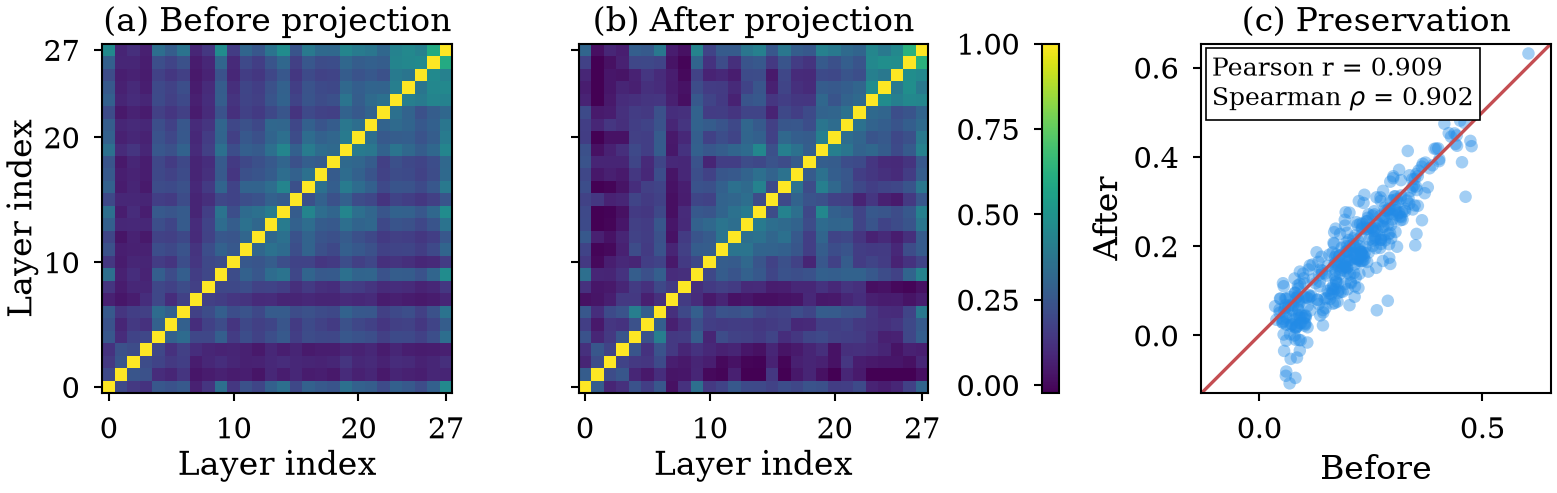
\includegraphics[width=0.9\linewidth]{Figures/figure5_projection_preservation.png}
    \caption{Feature structure preserved by the 64-dimensional column-orthogonal projection (Qwen2.5-VL-7B, LingoQA): pairwise similarity before vs. after projection.}
    \label{fig:jl}
\end{figure}

\begin{table}[!ht]
  \centering
  \caption{Nominal Inter-Layer Predictor performance on the group-disjoint 15\% predictor evaluation subset within the outer Training set.}
  \label{tab:fault_free_predictor_performance}
  \small
  \begin{tabular}{lcccccc}
    \toprule
    \multirow{2}{*}{Model}
      & \multicolumn{2}{c}{EarthVQA}
      & \multicolumn{2}{c}{LingoQA}
      & \multicolumn{2}{c}{VQAv2} \\
    \cmidrule(lr){2-3}
    \cmidrule(lr){4-5}
    \cmidrule(lr){6-7}
      & MSE & CosSim
      & MSE & CosSim
      & MSE & CosSim \\
    \midrule
    Qwen2.5-VL-7B
      & 0.0844 & 0.8589
      & 0.1451 & 0.7761
      & 0.2207 & 0.6934 \\
    InternVL3-8B
      & 0.0684 & 0.8117
      & 0.1094 & 0.7149
      & 0.1399 & 0.6367 \\
    LLaVA-1.5-7B
      & 0.0066 & 0.9138
      & 0.0162 & 0.7557
      & 0.0178 & 0.7326 \\
    \bottomrule
  \end{tabular}
\end{table}

\section{Configuration Selection}
\label{app:config}

\paragraph{Selection criterion.}
We select among 40 candidates spanning 4 feature dimensions and 10 window sizes. All candidates are evaluated only within the outer Training set via nested validation; the nine-task macro Significant-SDC F1 is the sole selection and ranking metric, and neither the internal Validation set nor the Test set participates. Figure~\ref{fig:config_matrix} (left) gives the complete 4$\times$10 matrix; the right panel re-scores the same candidate predictions against the fixed all-finite reference of the final 36D/$K{=}28$ configuration as an all-finite conditional diagnostic. Table~\ref{tab:A3} reports macro metrics at fixed $K{=}28$, and Figure~\ref{fig:window_ablation} gives window curves for both all retained executions and the all-finite subset at fixed 36D.

\begin{figure}[!ht]
\centering
    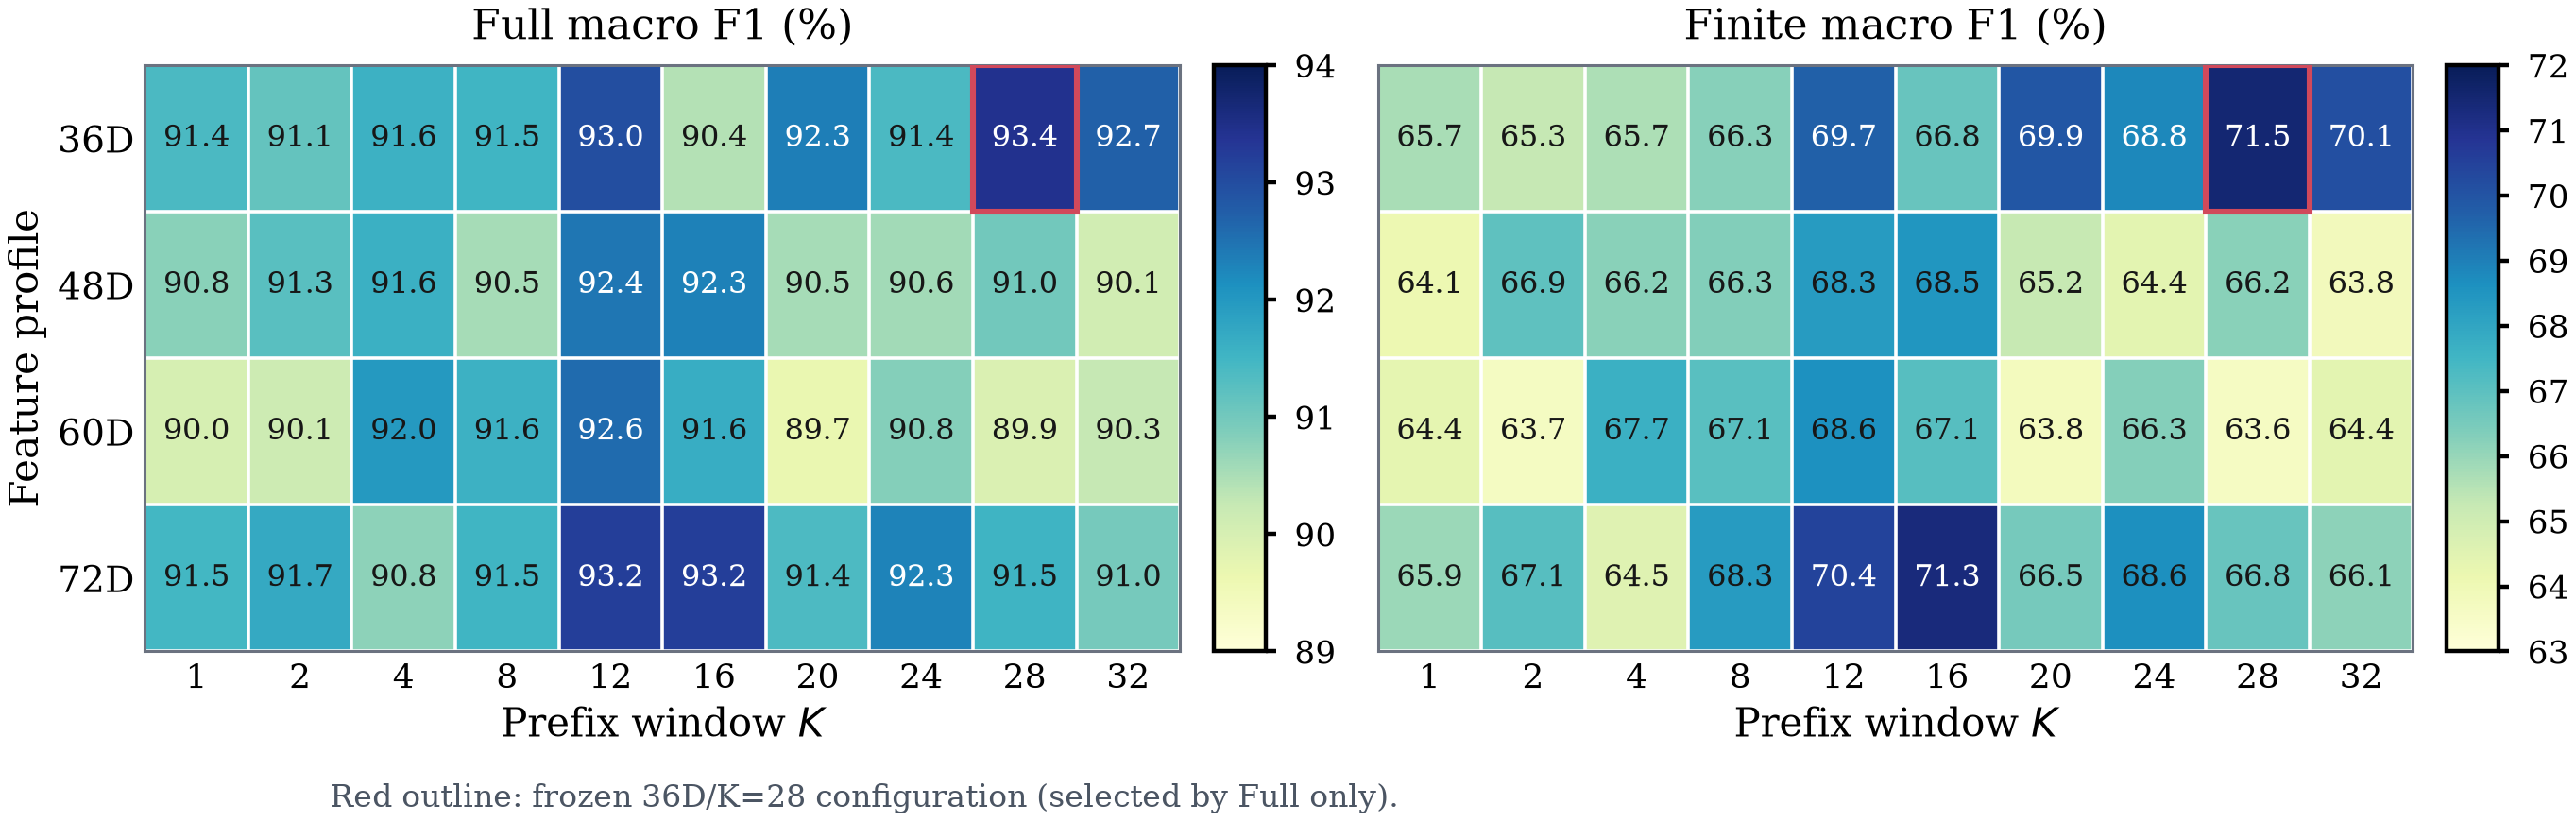
\includegraphics[width=1.0\linewidth]{Figures/figure8_configuration_F1_matrix.png}
    \caption{Training-only 4$\times$10 configuration-selection diagnostic. Left: nine-task macro Significant-SDC F1, the only result used for candidate selection and ranking; right: macro F1 scored on the fixed subset with all 36 features finite, after configuration freezing. Red boxes mark the 36D/$K{=}28$ selected and frozen by the primary metric; the two panels use independent color ranges.}
    \label{fig:config_matrix}
\end{figure}

\begin{table}[!ht]
\caption{Training-only macro metrics (\%) by feature dimension at fixed $K{=}28$.}
\label{tab:A3}
\centering
\small
\begin{tabular}{lcccc}
\toprule
\textbf{Feature} & \textbf{Precision} & \textbf{Recall} & \textbf{F1} & \textbf{FPR} \\
\midrule
\textbf{36D} & \textbf{99.17} & \textbf{88.66} & \textbf{93.42} & \textbf{0.028} \\
48D & 93.66 & 88.99 & 91.00 & 0.192 \\
60D & 92.77 & 88.22 & 89.93 & 0.270 \\
72D & 95.04 & 88.68 & 91.52 & 0.137 \\
\bottomrule
\end{tabular}
\end{table}

\begin{figure}[!ht]
\centering
    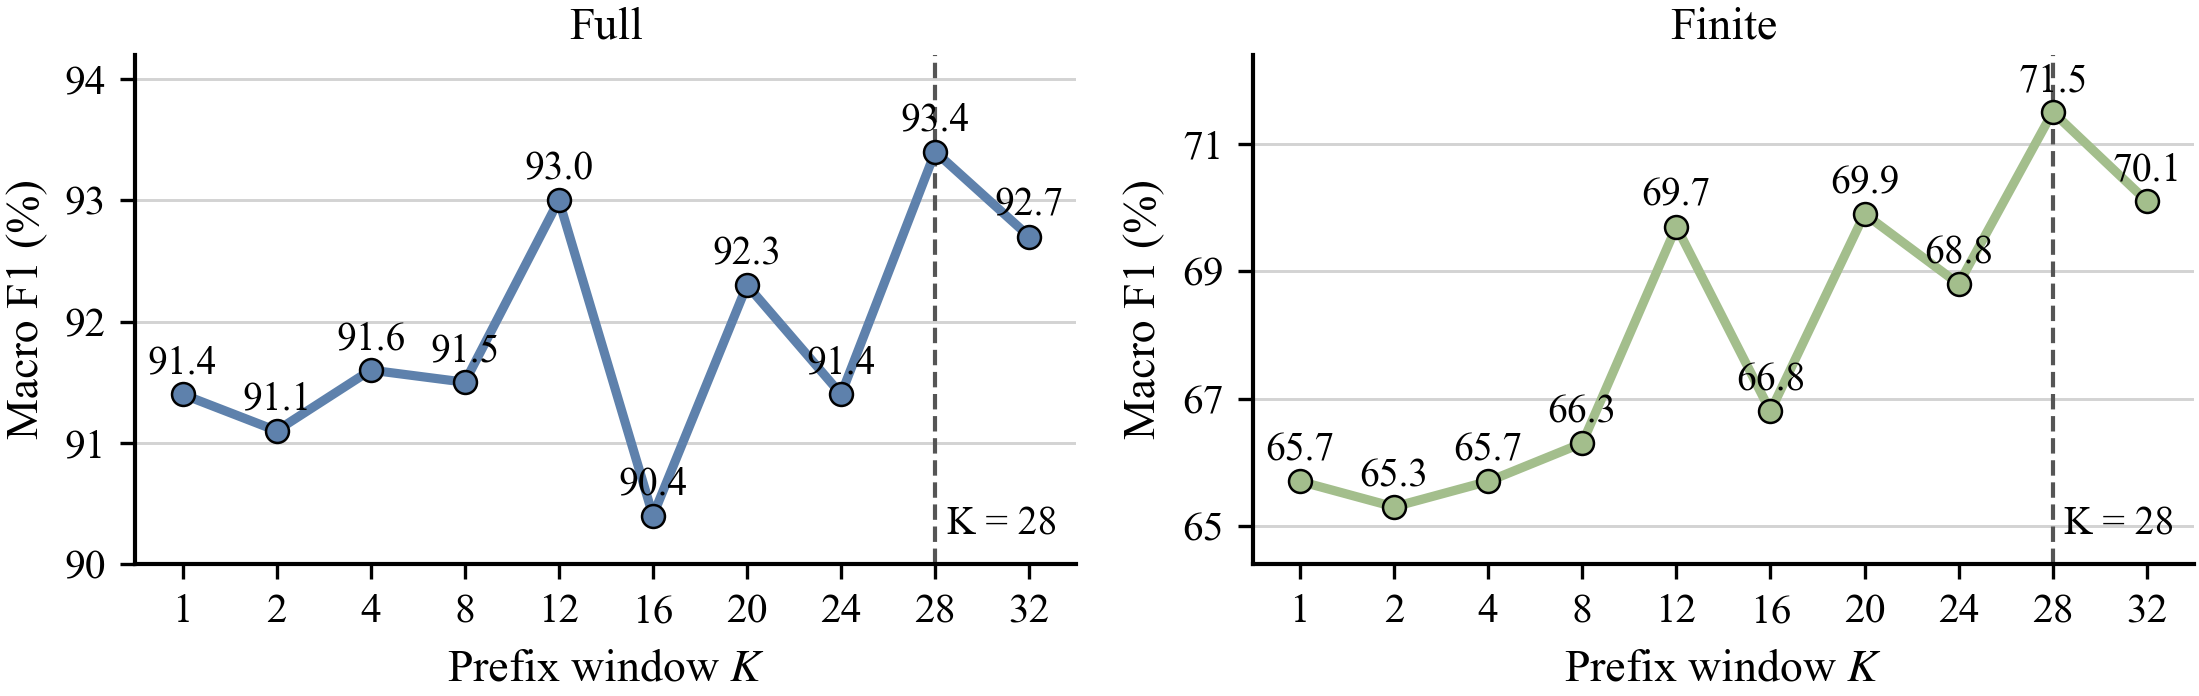
\includegraphics[width=1.0\linewidth]{Figures/figure9_window_ablation_F1.png}
    \caption{Training-only prefix-window diagnostic at fixed 36D. Left: macro F1; right: macro F1 scored on the fixed all-finite subset after configuration freezing. Each point is annotated with F1 (\%); dashed lines mark $K{=}28$ selected by the primary metric.}
    \label{fig:window_ablation}
\end{figure}

Fixed at $K{=}28$, 36D attains the highest F1 and the lowest FPR. The left panel of Figure~\ref{fig:window_ablation} shows that at fixed 36D, $K{=}28$ reaches the highest F1 (93.42\%); the right-side all-finite diagnostic likewise peaks at $K{=}28$ (71.49\%). We therefore freeze 36D/$K{=}28$, with the all-finite filter serving only as a post-freeze conditional diagnostic.

\paragraph{Post-freeze all-finite diagnostic.}
After configuration freezing, we run a conditional diagnostic within the same nested validation using the fixed 36D/$K{=}28$ all-finite reference vector. The filter changes only scored rows; training and threshold calibration are unchanged. Table~\ref{tab:A4} therefore explains performance under the numerically finite condition and plays no role in selecting or ranking the 40 candidates.

\begin{table}[!ht]
\caption{Training-only diagnostics of the frozen 36D/$K{=}28$ configuration on all retained executions and the all-finite subset (nine-task macro, \%).}
\label{tab:A4}
\centering
\small
\begin{tabular}{lcccccc}
\toprule
\textbf{Scope} & \textbf{Rows / Sig. SDC} & \textbf{Precision} & \textbf{Recall} & \textbf{F1} & \textbf{FPR} \\
\midrule
All & 53{,}076 / 1{,}912 & 99.17 & 88.66 & 93.42 & 0.028 \\
All-finite & 51{,}753 / 589 & 94.86 & 60.16 & 71.49 & 0.028 \\
\bottomrule
\end{tabular}
\end{table}

\section{Component Ablation Details}
\label{app:ablation}

Tables~\ref{tab:A5}--\ref{tab:A6} give the per-task F1 (\%) behind Figure~\ref{fig:ablation} in the main text. All variants are retrained, calibrated, and evaluated on the same nested partitions within the outer Training set; the outer Validation and Test sets do not participate. Table~\ref{tab:A5} covers all retained executions and is the primary result for component conclusions; Table~\ref{tab:A6} reports the conditional diagnostic on the fixed 36D/$K{=}28$ all-finite subset. The all-finite filter changes only scored rows; all variants are scored on the same subset, while thresholds remain frozen on the full internal Validation set. \texttt{-P} removes the 12 features of the corresponding layer pair; \texttt{-Cos/-Mean/-Std/-L2} removes the 9 features of that metric across all three pairs.

\begin{table}[!ht]
\caption{Per-task component ablation, Significant-SDC F1 on all retained executions (\%).}
\label{tab:A5}
\centering
\small
\resizebox{\ifdim\width>\textwidth\textwidth\else\width\fi}{!}{%
\begin{tabular}{lcccccccc}
\toprule
\textbf{Task} & \textbf{36D (all)} & \textbf{-P6/7} & \textbf{-P24/25} & \textbf{-P26/27} & \textbf{-Cos} & \textbf{-Mean} & \textbf{-Std} & \textbf{-L2} \\
\midrule
InternVL3-8B / EarthVQA & 97.02 & 97.05 & 97.37 & 97.20 & 97.04 & 96.85 & 97.19 & 97.02 \\
InternVL3-8B / LingoQA  & 98.15 & 98.14 & 98.60 & 98.75 & 91.93 & 98.14 & 98.14 & 98.29 \\
InternVL3-8B / VQAv2    & 96.70 & 96.70 & 96.12 & 95.45 & 94.86 & 96.27 & 96.27 & 96.27 \\
LLaVA-1.5-7B / EarthVQA & 96.85 & 95.45 & 96.85 & 96.47 & 95.69 & 96.88 & 96.09 & 96.88 \\
LLaVA-1.5-7B / LingoQA  & 91.60 & 84.21 & 85.11 & 78.43 & 90.77 & 72.73 & 90.23 & 91.95 \\
LLaVA-1.5-7B / VQAv2    & 92.70 & 92.24 & 81.06 & 88.52 & 92.24 & 84.71 & 92.70 & 84.71 \\
Qwen2.5-VL-7B / EarthVQA & 96.66 & 96.05 & 96.66 & 95.78 & 96.95 & 96.66 & 96.95 & 96.95 \\
Qwen2.5-VL-7B / LingoQA  & 87.58 & 87.93 & 87.58 & 87.42 & 82.66 & 82.90 & 85.55 & 82.32 \\
Qwen2.5-VL-7B / VQAv2    & 83.54 & 82.53 & 82.04 & 80.50 & 81.07 & 82.04 & 83.54 & 83.79 \\
\midrule
\textbf{Macro average} & \textbf{93.42} & \textbf{92.26} & \textbf{91.26} & \textbf{90.95} & \textbf{91.47} & \textbf{89.68} & \textbf{92.96} & \textbf{92.02} \\
\bottomrule
\end{tabular}%
}
\end{table}

\begin{table}[!ht]
\caption{Per-task component ablation, Significant-SDC F1 on the all-finite subset (\%).}
\label{tab:A6}
\centering
\small
\resizebox{\ifdim\width>\textwidth\textwidth\else\width\fi}{!}{%
\begin{tabular}{lcccccccc}
\toprule
\textbf{Task} & \textbf{36D (all)} & \textbf{-P6/7} & \textbf{-P24/25} & \textbf{-P26/27} & \textbf{-Cos} & \textbf{-Mean} & \textbf{-Std} & \textbf{-L2} \\
\midrule
InternVL3-8B / EarthVQA & 88.75 & 89.16 & 90.24 & 89.57 & 89.02 & 88.05 & 89.44 & 88.75 \\
InternVL3-8B / LingoQA  & 93.62 & 93.48 & 95.03 & 95.56 & 75.86 & 93.48 & 93.41 & 93.99 \\
InternVL3-8B / VQAv2    & 87.50 & 87.50 & 85.56 & 84.39 & 81.68 & 86.19 & 86.19 & 86.19 \\
LLaVA-1.5-7B / EarthVQA & 60.00 & 60.00 & 60.00 & 57.14 & 47.62 & 63.64 & 54.55 & 63.64 \\
LLaVA-1.5-7B / LingoQA  & 45.00 & 28.57 & 30.00 & 21.43 & 36.84 & 16.67 & 40.91 & 46.15 \\
LLaVA-1.5-7B / VQAv2    & 45.16 & 40.00 & 19.35 & 33.33 & 40.00 & 26.42 & 45.16 & 26.42 \\
Qwen2.5-VL-7B / EarthVQA & 89.32 & 87.38 & 89.32 & 86.79 & 90.20 & 89.32 & 90.20 & 90.20 \\
Qwen2.5-VL-7B / LingoQA  & 71.01 & 71.94 & 71.01 & 70.15 & 62.96 & 63.35 & 69.82 & 62.11 \\
Qwen2.5-VL-7B / VQAv2    & 63.01 & 61.33 & 60.53 & 54.41 & 58.97 & 60.53 & 63.01 & 63.45 \\
\midrule
\textbf{Macro average} & \textbf{71.49} & \textbf{68.82} & \textbf{66.78} & \textbf{65.86} & \textbf{64.80} & \textbf{65.29} & \textbf{70.30} & \textbf{68.99} \\
\bottomrule
\end{tabular}%
}
\end{table}

\section{Configuration-Matched Method Comparison}
\label{app:method}

Table~\ref{tab:A7} gives per-task Test-set Significant-SDC F1. Neither Ranger nor Dr.DNA provides a public implementation, so Ranger and Dr.DNA are configuration-matched adapted baselines that we re-implemented, not full reproductions of the original systems. The three methods use the same six monitored layers, the first $\min(28,T)$ actual decoding steps, the same fault instances and outer splits, and each selects its threshold on the full Validation set. Clean reference profiles for Ranger/Dr.DNA come from 20\% groups of the outer Training set, capped at 1{,}000 clean samples; SIEVE's Predictor uses the fault-free mapping telemetry of the outer Training set. The comparison therefore controls for monitoring scope, fault instances, and evaluation protocol, but does not claim identical clean-profiling budgets. The first three columns are the primary results covering all retained Test-set scored rows; the last three columns are the supplementary all-finite diagnostic under the same frozen evaluation. All scored rows are matched row-by-row by execution identity, output, and fault metadata.

\begin{table}[!ht]
\caption{Configuration-matched per-task Significant-SDC F1 (\%).}
\label{tab:A7}
\centering
\small
\resizebox{\ifdim\width>\textwidth\textwidth\else\width\fi}{!}{%
\begin{tabular}{lcccccc}
\toprule
\textbf{Task} & \textbf{Ranger (all)} & \textbf{Dr.DNA (all)} & \textbf{SIEVE (all)} & \textbf{Ranger (all-finite)} & \textbf{Dr.DNA (all-finite)} & \textbf{SIEVE (all-finite)} \\
\midrule
Qwen2.5-VL-7B / EarthVQA & 87.87 & 76.15 & 87.50 & 67.03 & 31.82 & 68.57 \\
Qwen2.5-VL-7B / LingoQA  & 64.91 & 61.33 & 96.10 & 32.81 & 15.79 & 86.67 \\
Qwen2.5-VL-7B / VQAv2    & 71.12 & 70.51 & 91.48 & 35.69 &  5.63 & 72.85 \\
InternVL3-8B / EarthVQA  & 90.49 & 86.96 & 98.61 & 69.06 & 40.24 & 94.65 \\
InternVL3-8B / LingoQA   & 76.13 & 82.17 & 95.40 & 41.51 & 14.55 & 83.33 \\
InternVL3-8B / VQAv2     & 82.25 & 79.95 & 94.38 & 28.83 & 13.04 & 82.32 \\
LLaVA-1.5-7B / EarthVQA  & 91.08 & 97.95 & 96.00 & 30.00 & 66.67 & 53.85 \\
LLaVA-1.5-7B / LingoQA   & 91.91 & 92.22 & 94.68 &  0.00 &  6.90 & 51.28 \\
LLaVA-1.5-7B / VQAv2     & 95.36 & 94.38 & 89.91 & 34.78 & 10.00 & 25.53 \\
\bottomrule
\end{tabular}%
}
\end{table}

\section{Online Overhead Details}
\label{app:overhead}

The overhead evaluation uses the final 36D/$K{=}28$ configuration: monitored pairs $(6,7)$, $(24,25)$, and $(26,27)$, over the first $\min(28,T)$ actual decoding steps. Each model--method pair runs 10 warmup and 10 forward repetitions on 50 LingoQA samples, yielding 500 observations; all monitored modes retain 100\% answer agreement.

\begin{table}[!ht]
\caption{LingoQA online overhead details. Latency in ms, overhead in \%.}
\label{tab:A8}
\centering
\small
\resizebox{\ifdim\width>\textwidth\textwidth\else\width\fi}{!}{%
\begin{tabular}{llrrrr}
\toprule
\textbf{Model} & \textbf{Method} & \textbf{Mean} & \textbf{P50} & \textbf{P95} & \textbf{Overhead} \\
\midrule
\multirow{4}{*}{Qwen2.5-VL-7B}
 & No Detection   & 764.4  & 727.0  & 951.3  & 0.00 \\
 & Ranger   & 777.9  & 738.9  & 971.2  & 1.77 \\
 & Dr.DNA   & 793.6  & 753.8  & 995.5  & 3.82 \\
 & SIEVE          & 813.7  & 773.1  & 1025.6 & 6.44 \\
\midrule
\multirow{4}{*}{InternVL3-8B}
 & No Detection   & 984.3  & 932.5  & 1374.9 & 0.00 \\
 & Ranger   & 1001.8 & 948.9  & 1397.2 & 1.78 \\
 & Dr.DNA   & 1035.5 & 981.2  & 1446.3 & 5.20 \\
 & SIEVE          & 1048.7 & 992.7  & 1460.4 & 6.53 \\
\midrule
\multirow{4}{*}{LLaVA-1.5-7B}
 & No Detection   & 363.8  & 249.3  & 640.8  & 0.00 \\
 & Ranger   & 373.9  & 254.1  & 663.8  & 2.75 \\
 & Dr.DNA   & 384.5  & 258.4  & 689.5  & 5.67 \\
 & SIEVE          & 389.2  & 263.2  & 698.5  & 6.98 \\
\bottomrule
\end{tabular}%
}
\end{table}

\section{Detector Transfer}
\label{app:transfer}

We evaluate the $9\times9$ transfer of the frozen 36D/$K{=}28$ SIEVE Detector, with target-specific clean Mapping, across the nine model--dataset tasks. For each source $\rightarrow$ target cell, the Detector and its maximum-F1 threshold are trained and frozen on the source's Training/Validation; the target trains its Mapping only on its own fault-free executions and generates 36D Test-set features. Target Training/Validation fault labels play no role in Detector training, threshold calibration, or tuning, and target Test-set labels are used only for offline scoring. All tasks use the same random dual-bit injections, with telemetry recorded for up to 50 decoding steps. The all-finite subset requires all 36 features of target Test-set executions to be finite, serving only as a conditional diagnostic without changing predictions, models, or thresholds.

\begin{figure}[!ht]
\centering
    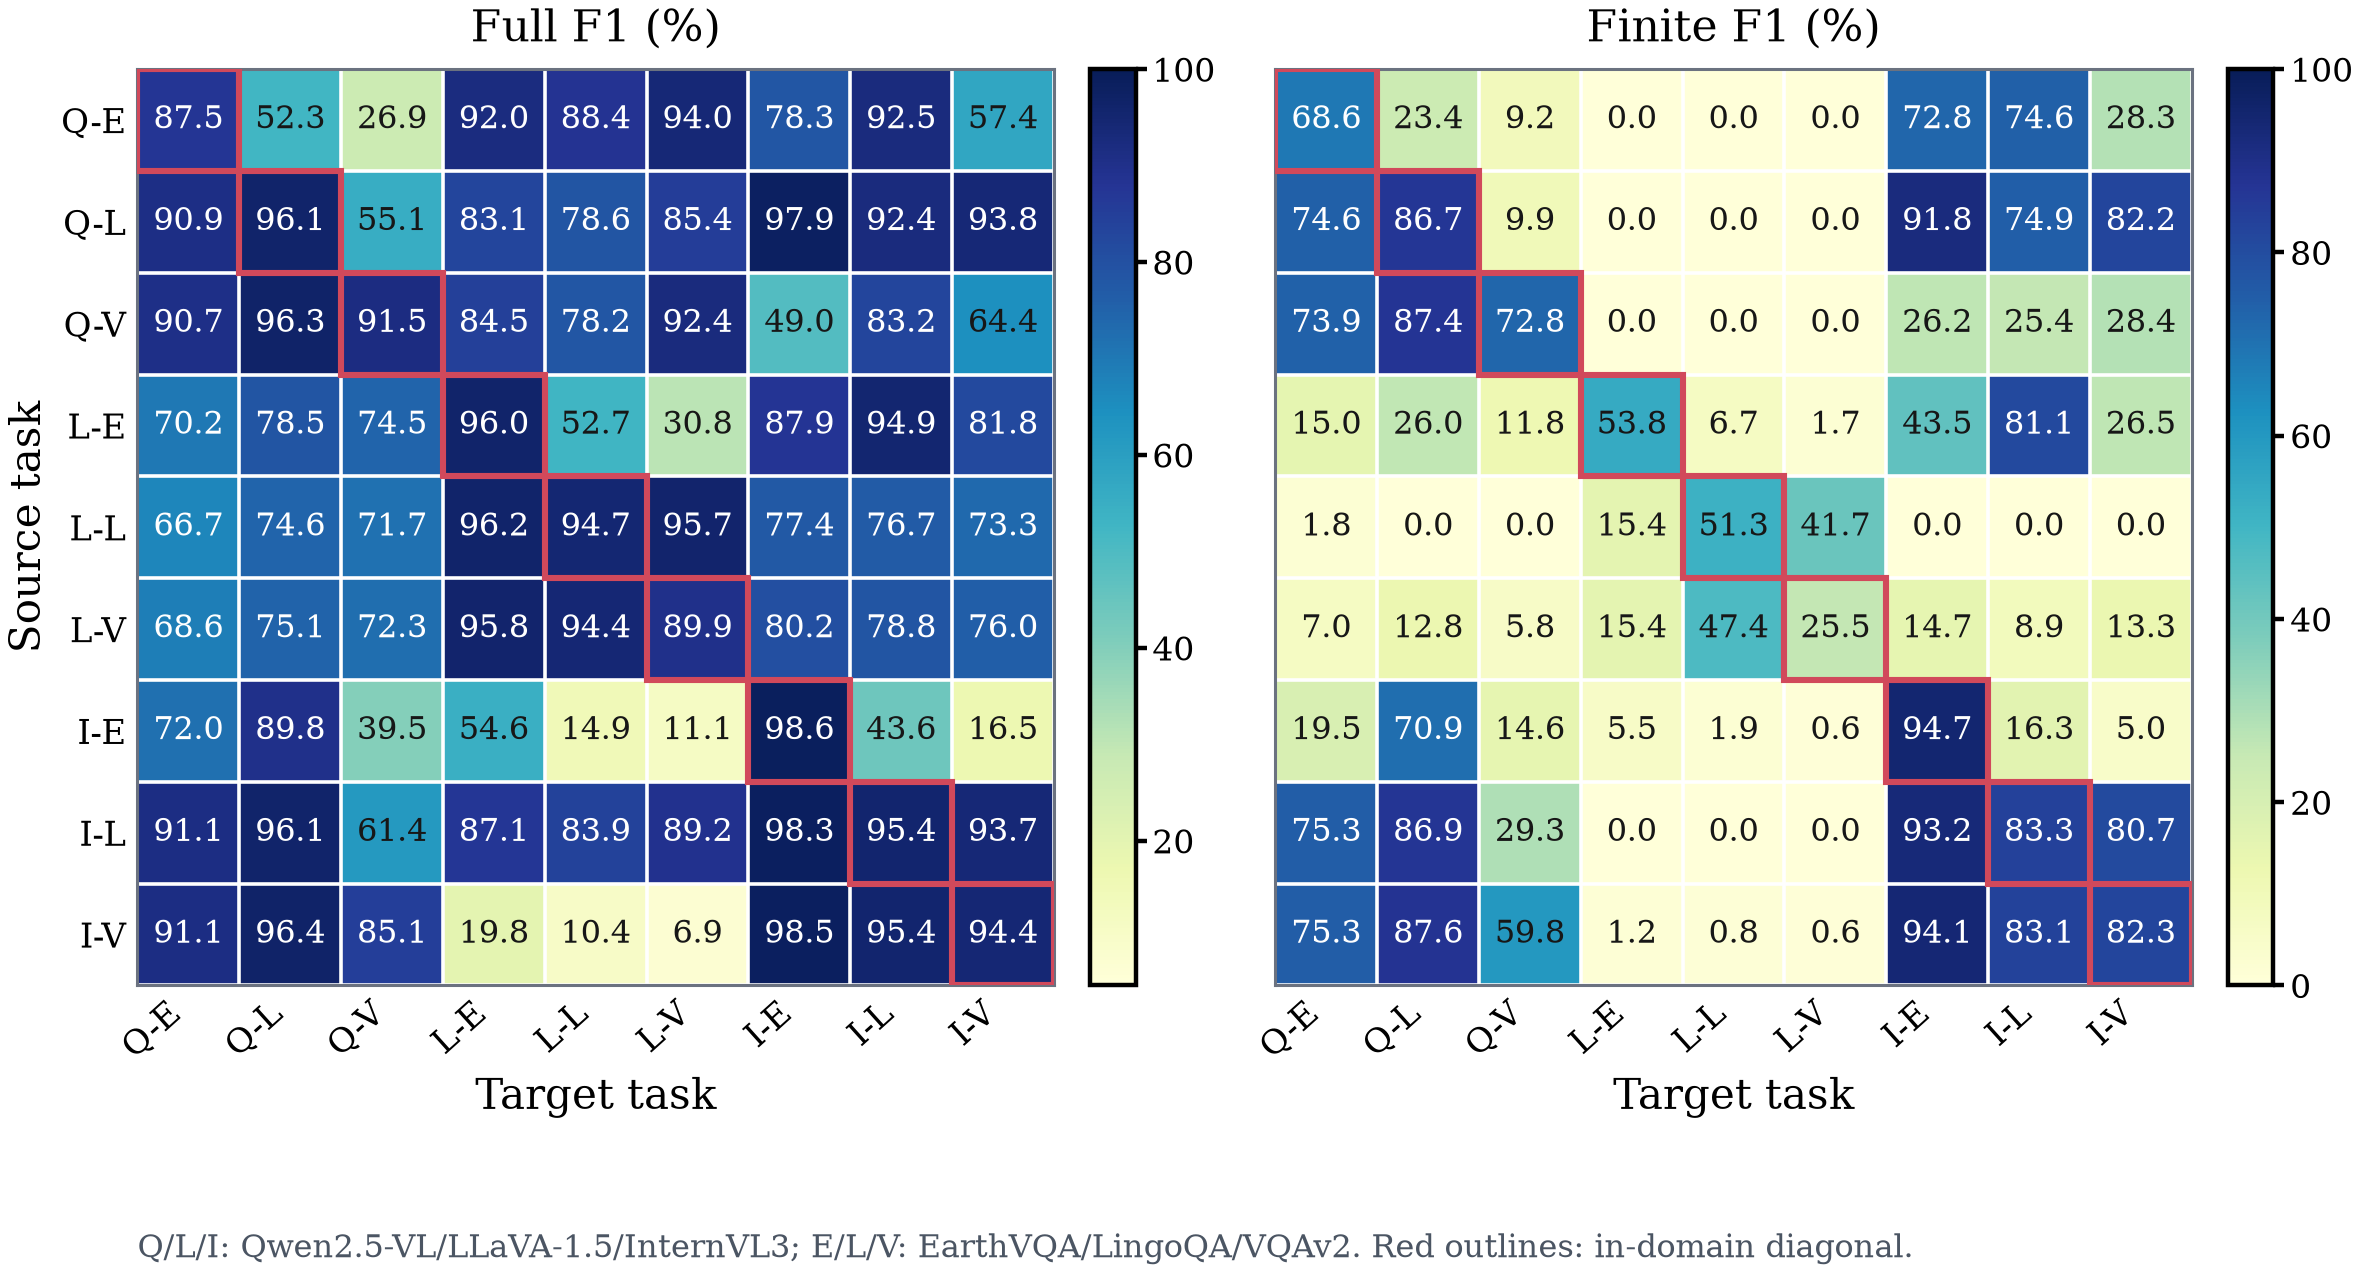
\includegraphics[width=1.0\linewidth]{Figures/figure10_transfer_F1_matrix.png}
    \caption{$9\times9$ transfer F1 (\%) of the frozen 36D/$K{=}28$ Detector. Rows are sources, columns are targets; source Detectors and thresholds are fixed, and each target uses only its own clean Mapping to generate features. Left: all retained executions; right: all-finite conditional diagnostic after configuration freezing. Red boxes mark the in-domain diagonal. Q/L/I denote Qwen2.5-VL, LLaVA-1.5, InternVL3; E/L/V denote EarthVQA, LingoQA, VQAv2.}
    \label{fig:transfer}
\end{figure}

The nine diagonal cells in Figure~\ref{fig:transfer} (all retained executions) reproduce the \S4.2.1 Test-set results item by item (macro F1 $=$ 93.78\%). Across the 72 off-diagonal cells, the macro F1 is 73.46\% with an FPR of 3.97\%, clearly higher than the 0.11\% in-domain; the macro F1 on the all-finite subset is 28.91\%, a supplementary diagnostic under fixed conditions. These results indicate that some source--target combinations transfer, but a target-specific clean Mapping remains necessary, and there is a substantial calibration mismatch between the frozen source threshold and the target distribution; this does not constitute evidence of zero-shot deployment without target-side data.

\begin{table}[!ht]
\caption{Macro-averaged Significant-SDC metrics (\%) by transfer relationship, all retained executions.}
\label{tab:A9}
\centering
\small
\begin{tabular}{lccccc}
\toprule
\textbf{Relationship} & \textbf{Cells} & \textbf{Precision} & \textbf{Recall} & \textbf{F1} & \textbf{FPR} \\
\midrule
In-domain & 9 & 96.38 & 91.49 & 93.78 & 0.11 \\
Same model, cross dataset & 18 & 71.95 & 89.14 & 73.55 & 5.81 \\
Cross model, same dataset & 18 & 90.06 & 72.64 & 75.24 & 3.19 \\
Cross model, cross dataset & 36 & 84.07 & 75.66 & 72.53 & 3.45 \\
\midrule
\textbf{Off-diagonal macro} & \textbf{72} & \textbf{82.54} & \textbf{78.28} & \textbf{73.46} & \textbf{3.97} \\
\bottomrule
\end{tabular}
\end{table}

\begin{table}[!ht]
\caption{Macro-averaged Significant-SDC metrics (\%) by transfer relationship, all-finite subset.}
\label{tab:A10}
\centering
\small
\begin{tabular}{lccccc}
\toprule
\textbf{Relationship} & \textbf{Cells} & \textbf{Precision} & \textbf{Recall} & \textbf{F1} & \textbf{FPR} \\
\midrule
In-domain & 9 & 79.88 & 62.81 & 68.78 & 0.11 \\
Same model, cross dataset & 18 & 62.09 & 54.09 & 43.28 & 5.81 \\
Cross model, same dataset & 18 & 49.68 & 25.53 & 23.67 & 3.19 \\
Cross model, cross dataset & 36 & 48.16 & 29.52 & 24.35 & 3.45 \\
\midrule
\textbf{Off-diagonal macro} & \textbf{72} & \textbf{52.02} & \textbf{34.66} & \textbf{28.91} & \textbf{3.97} \\
\bottomrule
\end{tabular}
\end{table}

Each matrix cell is bootstrapped 10{,}000 times over the target's image/question groups; per-cell F1 and 95\% CIs are provided with the accompanying reproduction results. Because the same source threshold is applied directly to different target distributions, the off-diagonal FPR and performance gaps reflect the actual transfer calibration mismatch rather than a re-selected operating point.

\section{Limitations}
\label{app:limitations}

Our conclusions are bounded by prefill-stage random dual-bit injection, fixed-rubric LLM-as-a-Judge labels, and target-side clean Mapping telemetry; detector transfer shows calibration mismatch across tasks rather than zero-shot deployability. Future work includes manual label audits, robustness to diverse fault models, and integration with recovery mechanisms.

\end{document}
